\documentclass[journal,onecolumn,10pt]{IEEEtran}

\usepackage{cite}
\usepackage{amsmath,amssymb,amsfonts}
\usepackage{graphicx}
\usepackage{textcomp}
\usepackage{booktabs}
\usepackage{needspace}
\usepackage{longtable}
\usepackage{float,needspace}
\usepackage{capt-of}
\renewcommand{\thetable}{S\arabic{table}}
\renewcommand{\theequation}{S\arabic{equation}}
\usepackage{calc}
\usepackage{tabularx}
\usepackage{array}
\usepackage{multirow}
\usepackage{url}
\usepackage{stfloats}
\usepackage{balance}
\usepackage[hidelinks]{hyperref}
\providecommand{\tightlist}{\setlength{\itemsep}{0pt}\setlength{\parskip}{0pt}}
\hyphenation{LoRaWAN local-iza-tion re-ceiv-er}

\graphicspath{{../figures/}{figures/}}
\renewcommand{\thefigure}{S\arabic{figure}}
\hypersetup{pdftitle={Supplementary Material: Recalibration Can Mask Measured Sensitivity to Receiver-Coordinate Errors in RSSI Localization},pdfauthor={Ananta Ranjan and Vijay Kumar Jha},pdfsubject={Receiver-coordinate perturbation study: supporting methods and source evidence},pdfkeywords={RSSI localization, receiver-coordinate error, LoRaWAN, robustness}}

\graphicspath{{figures/}{./}}
\begin{document}
\title{Supplementary Material for: Recalibration Can Mask Measured Sensitivity to Receiver-Coordinate Errors in RSSI Localization}
\author{Ananta Ranjan and Vijay Kumar Jha}
\maketitle
This supplement reports the complete controlled-perturbation grids, reference-substrate safeguards, dependence analyses, and provenance needed to interpret the main article. Raw logs and machine-readable tables are indexed in the accompanying computational evidence package. 

\noindent\textbf{Author Contributions.} Ananta Ranjan: conceptualization, methodology, software, validation, formal analysis, investigation, resources, data curation, writing---original draft, visualization, and project administration. Vijay Kumar Jha: supervision and writing---review and editing.

\noindent\textbf{Funding.} No funding was received for this work.

\noindent\textbf{Conflict of interest.} None of the authors have a conflict of interest to disclose.

\noindent\textbf{AI-assisted tool disclosure.} During this study and preparation of the manuscript, the authors used ChatGPT Sol 5.6 to assist with source-code inspection, code debugging, numerical consistency checks, analysis of computational outputs, and revision of the manuscript and supplementary material, and to assist with initial drafting and language revision. The authors directed these activities and repeatedly reviewed the AI-assisted work against the study's methods, computational records, and research objectives, checking implementation correctness and completeness and evaluating interpretations against the available evidence. The authors determined which suggestions to adopt, revise, or reject, made the final methodological and interpretive decisions, and take full responsibility for the manuscript and supplementary material.

\noindent\textbf{Review evidence access.} The version-matched computational package is version 1.1.0, identified by DOI \url{https://doi.org/10.5281/zenodo.23061691} and mirrored in the GitHub repository. It supplies the frozen baseline inputs and outputs, the complete 32-field paired-calibration intervention, numerical diagnostic tables, source records and read-only verification entry points. The corresponding release asset is \path{PAPERB_SENSORS_EVIDENCE_v1.1.0_S8_300926.zip}. The preceding version 1.0.0 baseline remains at \url{https://doi.org/10.5281/zenodo.22680802}; that earlier DOI does not identify the new extension. Source observations are obtained separately from the fingerprinted public release.


\section*{S1. Dataset, population, and run controls}\label{s1.-dataset-population-and-run-controls}

\begin{center}\begin{minipage}{\textwidth}\centering
\captionof{table}{S1. Dataset, population, and run controls}

\begin{tabular}{@{}
  >{\raggedright\arraybackslash}p{(\columnwidth - 4\tabcolsep) * \real{0.2426}}
  >{\raggedright\arraybackslash}p{(\columnwidth - 4\tabcolsep) * \real{0.1838}}
  >{\raggedright\arraybackslash}p{(\columnwidth - 4\tabcolsep) * \real{0.5735}}@{}}
\toprule\noalign{}
\begin{minipage}[b]{\linewidth}\raggedright
Component
\end{minipage} & \begin{minipage}[b]{\linewidth}\raggedright
Setting
\end{minipage} & \begin{minipage}[b]{\linewidth}\raggedright
Scope
\end{minipage} \\
\midrule\noalign{}

Primary population & Antwerp LoRaWAN v1.3 & Parsed 130,429 records; 55,375 with \textgreater=3 receptions \\
Calibration/evaluation & Frozen 30/70 split & 16,612 calibration; 2,498 fixed evaluation after 2 duplicate records removed \\
Reference geometry & Recovered-29 & Correlation-audited; not independently surveyed; all 29 labels join \\
Standard receiver window & max\_gws=10 & At least 3 mapped and calibrated receptions before selection \\
Perturbed receiver window & max\_gws=5 & Separate redraw references measured \\
Estimators & WCL, ABS, DIFF, Min-Max & Four implemented pipelines; ABS/DIFF share bounded WCL-centered search \\
Standard redraw references & ABS instrument & 4.5\% evaluation redraw; 1.4\% calibration redraw \\
Five-receiver redraw references & ABS instrument & 4.7\% evaluation redraw; 1.6\% calibration redraw \\
DIFF pair rule & tau=3 dB & If fewer than 2 pairs survive, score all available pairs \\
\bottomrule
\end{tabular}
\end{minipage}\end{center}

The primary recovered-29 localization runs use the fixed 2,498-message evaluation population after two content-duplicate records are removed; the native and common-roster B9C controls use the separately identified populations in Section S12 and the repository population manifests. Recovered-29 is correlation-audited rather than independently surveyed. Every map-dependent result therefore remains conditional on that reference geometry. Throughout the supplement, a negative percentage change denotes a lower median localization error than the fixed reference, not a negative distance. Because the fixed recovered geometry is an experimental reference rather than an estimator-specific optimum, some perturbation directions can produce small apparent improvements.

The released transmitter coordinates provide the reference for calibration distances and localization-error scoring; their physical accuracy was not independently established in this study. Exact-content deduplication does not exclude nearby or repeated campaign locations across the random split. The matched effects are conditional within-campaign comparisons, not spatially or temporally independent deployment validation.

\subsection*{S1.1 Exact reconstruction and implemented pipeline}
The table below fixes eligibility and scoring. Ordered zero-based original CSV data-row indices are stored in the population manifests under \path{results/rc5/populations/}. They are not indices into the filtered 55,375-message table. The coordinate assignment CSV supplies all 233 entries across the eight maps, in EPSG:32631 metres; map-byte hashes and ordered-population hashes are in the manifests. This does not certify a surveyed physical coordinate truth.
\begin{center}\begin{minipage}{\textwidth}\centering\small
\captionof{table}{Essential population and implementation rules.}\label{tab:s-exact-methods}
\begin{tabular}{@{}p{.21\textwidth}p{.74\textwidth}@{}}
\toprule
Operation & Executed rule \\
\midrule
Input and projection & Pinned LoRaWAN v1.3 CSV; finite BS values in [-150,-20] dBm. No HDOP filter. Longitude/latitude (EPSG:4326, longitude first) to UTM 31N (EPSG:32631). \\
Working set and split & Retain source-row order, require at least three valid receptions, shuffle with Python \texttt{Random(1)}; first $\lfloor0.3N\rfloor$ messages calibrate. \\
Evaluation sample & Require at least three active-roster receptions in the remaining pool; \texttt{Random(9).sample} selects up to 2,500. Remove keys matching a calibration record. \\
Content key & Tuple of projected $(x,y)$ rounded to three decimals and sorted tuples of (receiver ID, RSSI rounded to three decimals). The full reception set enters the key. \\
Calibration filter & At least ten calibration receptions per receiver; otherwise no $A_0$. Filter mapped-and-calibrated receivers before strongest-RSSI selection. Fewer than three leaves no estimate. \\
Selection ties & Per-message strongest raw RSSI, preserving source BS-column order on a tie; maximum ten (or five in its named sensitivity). Global exposure-count ties use numeric receiver ID. \\
ABS/DIFF search & WCL initialization; axis-aligned square side/spacing (6000,600) m then (1500,150) m. Triangular rows advance by $s\sqrt{3}/2$, alternating a half-spacing in x. Increasing y, then x; first enumerated minimum wins ties. Fine square centers at coarse minimum. \\
Coordinate adaptation & Fresh map-specific median intercept fit after each perturbation, unless the WCL frozen-$A_0$ ablation is named. DIFF admits corrected-RSSI pairs at 3 dB; fewer than two admitted pairs triggers all pairs. \\
Perturbation coupling & Top-$k$ seeds $8800+k+101r$ differ across $k$. Matched exposure uses one field per subset. Legacy rotation control seeds $4750+13r$; operational exact-profile seeds $7750+13r$ for $r=0,\ldots,7$. \\
Summary semantics & Primary: median over perturbation-level message medians. Min--max describes the retained perturbations. Dependence: difference of medians of per-message direction medians (S13), conditional on those fields. \\
\bottomrule
\end{tabular}
\end{minipage}\end{center}

\noindent\textit{Calibration constraints.} With $n$ fixed, each eligible receiver's intercept is the separately computed median specified in main Equation~(4). No intercept bounds, clipping, regularization or cross-receiver intercept-parameter sharing is applied. The minimum of ten calibration receptions is an eligibility rule, not a constraint on intercept values. These choices are unchanged in the refitted arm of S17.

\subsection*{S1.2 Eight roster constructions and absolute reference medians}
\begin{center}\begin{minipage}{\textwidth}\centering\small
\captionof{table}{References at $n=4.7$, receiver window ten. Min. cal. is the smallest per-receiver calibration count. No receiver triggers the ten-observation exclusion in these frozen populations.}\label{tab:s-baselines}
\begin{tabular}{@{}lrrrrrrr@{}}
\toprule
Substrate & $G$ & $N$ & Min. cal. & WCL (m) & ABS (m) & DIFF (m) & Min-Max (m) \\
\midrule
R29 & 29 & 2498 & 30 & 597.67 & 641.01 & 963.95 & 466.01 \\
O32$-$71 & 32 & 2498 & 46 & 593.74 & 555.62 & 1082.71 & 478.88 \\
O33 published & 33 & 2495 & 46 & 584.75 & 527.75 & 1011.54 & 467.64 \\
O33 substituted & 33 & 2495 & 46 & 579.95 & 527.52 & 1012.57 & 465.81 \\
R27 & 27 & 2498 & 58 & 593.22 & 639.99 & 989.62 & 469.82 \\
O27 & 27 & 2498 & 58 & 550.15 & 560.26 & 1104.03 & 442.66 \\
R26 & 26 & 2494 & 69 & 613.74 & 644.48 & 1001.08 & 509.64 \\
O26 & 26 & 2494 & 69 & 577.00 & 549.19 & 1048.15 & 480.57 \\
\bottomrule
\end{tabular}
\end{minipage}\end{center}
R29 is the frozen historical correlation-selected reference, with the audit and selection-history limitations stated in S15. O33 published retains all 33 catalogue pairs; O33 substituted replaces only BS71 by its R29 value. O32$-$71 removes BS71 from the catalogue map. R27 restricts R29 to the common identities; \textbf{O27 restricts the substituted-71 map}, so only its other 26 coordinates are catalogue-derived and BS71 is identical in both arms. R26/O26 additionally omit BS71. Ordered messages match within each common-roster pair, not generally across native rosters. These are the unchanged executed constructions; the \texttt{official27} filename does not denote a fully unrepaired catalogue subset. All reference fits and baseline arrays predate this documentary revision. The no-exclusion check is limited to the frozen calibration split.

\section*{S2. Corruption-load surface}\label{s2.-paper-b-exclusive-corruption-load-surface}

The first column gives the exact number of corrupted receivers out of 29, not a rounded percentage. The tables display the five expansion magnitudes used in the main figure. The earlier 5-km fraction slice is retained, with its source, population, randomization and recalibration rules, in S16. Its inclusion there is historical continuity and reporting, not new execution or reassignment of novelty from another manuscript.

\Needspace{6\baselineskip}
\subsection*{S2.1 WCL median-error change (\%)}\label{s2.1-wcl-median-error-change}

\begin{center}\begin{minipage}{\textwidth}\centering
\captionof{table}{S2.1 WCL median-error change (\%)}

\begin{tabular}{@{}rrrrrr@{}}
\toprule\noalign{}
Corrupted count & 250\_m & 500\_m & 1000\_m & 2500\_m & 10000\_m \\
\midrule\noalign{}

1 & 0.0 & 0.0 & 0.0 & 0.1 & 0.1 \\
3 & 0.4 & 0.2 & 3.8 & 4.1 & 4.0 \\
7 & -0.4 & 0.1 & 6.3 & 17.2 & 18.1 \\
14 & 0.8 & 11.4 & 22.6 & 46.8 & 53.3 \\
21 & 10.1 & 20.2 & 38.5 & 75.3 & 134.8 \\
29 & 2.8 & 14.0 & 45.3 & 155.9 & 845.2 \\
\bottomrule
\end{tabular}
\end{minipage}\end{center}

\Needspace{6\baselineskip}
\subsection*{S2.2 ABS median-error change (\%)}\label{s2.2-abs-median-error-change}

\begin{center}\begin{minipage}{\textwidth}\centering
\captionof{table}{S2.2 ABS median-error change (\%)}

\begin{tabular}{@{}rrrrrr@{}}
\toprule\noalign{}
Corrupted count & 250\_m & 500\_m & 1000\_m & 2500\_m & 10000\_m \\
\midrule\noalign{}

1 & 0.0 & 0.0 & 0.1 & 0.2 & 0.6 \\
3 & 0.1 & 0.2 & 3.8 & 4.5 & 6.3 \\
7 & -0.6 & 1.2 & 7.4 & 8.5 & 10.0 \\
14 & -0.5 & 4.5 & 10.0 & 15.6 & 37.0 \\
21 & 0.8 & 8.6 & 14.2 & 31.5 & 80.2 \\
29 & 0.5 & 11.6 & 40.1 & 78.1 & 369.8 \\
\bottomrule
\end{tabular}
\end{minipage}\end{center}

\Needspace{6\baselineskip}
\subsection*{S2.3 DIFF median-error change (\%)}\label{s2.3-diff-median-error-change}

\begin{center}\begin{minipage}{\textwidth}\centering
\captionof{table}{S2.3 DIFF median-error change (\%)}

\begin{tabular}{@{}rrrrrr@{}}
\toprule\noalign{}
Corrupted count & 250\_m & 500\_m & 1000\_m & 2500\_m & 10000\_m \\
\midrule\noalign{}

1 & -0.1 & 0.0 & 0.1 & 0.0 & -0.8 \\
3 & 1.5 & 1.3 & 4.1 & 2.8 & 0.1 \\
7 & 0.6 & 4.1 & 9.5 & 11.5 & -1.7 \\
14 & 2.5 & 9.9 & 1.4 & 16.9 & 14.8 \\
21 & 16.5 & 12.6 & 37.3 & 35.5 & 58.7 \\
29 & 5.9 & 15.8 & 43.8 & 67.9 & 242.9 \\
\bottomrule
\end{tabular}
\end{minipage}\end{center}

\Needspace{6\baselineskip}
\subsection*{S2.4 Min-Max median-error change (\%)}\label{s2.4-min-max-median-error-change}

\begin{center}\begin{minipage}{\textwidth}\centering
\captionof{table}{S2.4 Min-Max median-error change (\%)}

\begin{tabular}{@{}rrrrrr@{}}
\toprule\noalign{}
Corrupted count & 250\_m & 500\_m & 1000\_m & 2500\_m & 10000\_m \\
\midrule\noalign{}

1 & 0.1 & 0.0 & 0.0 & 0.2 & 0.1 \\
3 & 0.3 & 1.3 & 2.9 & 4.2 & 17.8 \\
7 & -0.7 & 1.7 & 7.2 & 19.5 & 50.8 \\
14 & 1.3 & 10.4 & 15.2 & 41.2 & 97.0 \\
21 & 1.7 & 13.2 & 32.8 & 65.8 & 209.2 \\
29 & 1.6 & 15.9 & 47.4 & 127.1 & 582.9 \\
\bottomrule
\end{tabular}
\end{minipage}\end{center}

\section*{S3. Exposure-ranked receiver sets}\label{s3.-exposure-ranked-receiver-sets}

The table below reports the direction-replicated 5-km top-k branch. The review package supplies all central branches and the retained top-/bottom-k ranges. Historical individual random-k ranges were not retained and are explicitly marked unavailable, not inferred from their central values (S14.6).

\begin{center}\begin{minipage}{\textwidth}\centering
\captionof{table}{S3. Exposure-ranked receiver sets}

\begin{tabular}{@{}rrrrrr@{}}
\toprule\noalign{}
k & S & WCL\_pct & ABS\_pct & DIFF\_pct & MinMax\_pct \\
\midrule\noalign{}

1 & 0.0961 & 3.6 & 1.8 & -4.8 & 17.2 \\
2 & 0.1866 & 1.5 & 7.8 & -5.6 & 35.1 \\
3 & 0.2680 & 27.4 & 13.4 & 2.6 & 44.7 \\
4 & 0.3398 & 43.2 & 28.9 & 9.1 & 66.1 \\
5 & 0.4088 & 44.6 & 28.0 & 10.7 & 67.3 \\
6 & 0.4768 & 49.5 & 38.2 & 13.4 & 98.0 \\
7 & 0.5348 & 233.4 & 65.0 & 48.8 & 243.3 \\
8 & 0.5860 & 220.6 & 69.0 & 39.9 & 220.1 \\
9 & 0.6355 & 197.5 & 67.9 & 41.3 & 184.1 \\
10 & 0.6818 & 282.6 & 82.5 & 50.0 & 242.8 \\
11 & 0.7263 & 282.6 & 83.4 & 52.8 & 238.0 \\
12 & 0.7693 & 344.1 & 105.9 & 68.3 & 267.4 \\
13 & 0.8116 & 303.6 & 100.3 & 75.4 & 310.8 \\
14 & 0.8394 & 346.1 & 112.3 & 72.7 & 304.6 \\
\bottomrule
\end{tabular}
\end{minipage}\end{center}

\Needspace{6\baselineskip}
\subsection*{S3.1 Approximately matched exposure configurations}\label{s3.1-matched-exposure-falsifier}

For the fixed reference-selected receiver sets $G_q$, define
\begin{equation}\label{eq:s-exposure}
S(T)=\frac{\sum_q |G_q\cap T|}{\sum_q|G_q|},\qquad \sum_q|G_q|=10{,}680.
\end{equation}
A continuous Python \texttt{Random(6606)} stream proposes $k\in\{2,\ldots,14\}$ and a uniform $k$-subset of numerically ordered receiver IDs. For each center 0.10, 0.20, 0.30, 0.40 or 0.50, accept the first eight subsets with $|S-S_{\rm center}|\le0.025$ (maximum 4,000 proposals). Each accepted subset receives one 5-km independent-direction field, generated by \texttt{default\_rng(6700+j)} for within-bin index $j=0,\ldots,7$; $j$ resets in each bin. Directions are consumed in numeric receiver order, only for targeted receivers. There is \emph{one}, not eight, direction realization per subset, so within-subset directional variation is not estimated.

The original block retained bin aggregates rather than individual scores. The RC5 reporting-recovery script re-executed these same 40 configurations without changing code or seeds and exported all four methods' message-level errors. All 30 printed aggregate fields reproduce at one-decimal precision. These new exports are labelled assistant-runtime reporting derivatives, not historical per-subset records or new confirmatory experiments.


\begin{figure}[H]
\centering
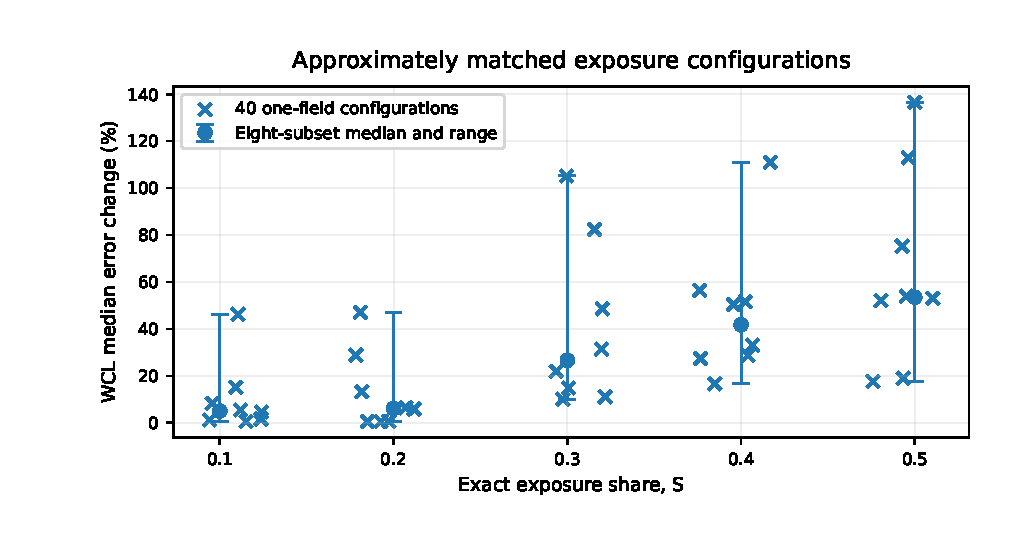
\includegraphics[width=0.88\textwidth]{FigS1_Matched_Exposure.pdf}
\caption{Forty approximately matched exposure configurations. Points use exact exposure shares; bin summaries use eight subsets each. Subset identity, count, exact share and one direction field vary jointly. Bars are configuration ranges, not confidence intervals or isolated co-occurrence effects.}
\end{figure}

\begin{center}\begin{minipage}{\textwidth}\centering\small
\renewcommand{\arraystretch}{1.18}\setlength{\tabcolsep}{4pt}
\captionof{table}{S3.1 Approximately matched exposure configurations}

\begin{tabular}{@{}
  >{\raggedleft\arraybackslash}p{(\columnwidth - 14\tabcolsep) * \real{0.1176}}
  >{\raggedleft\arraybackslash}p{(\columnwidth - 14\tabcolsep) * \real{0.1176}}
  >{\centering\arraybackslash}p{(\columnwidth - 14\tabcolsep) * \real{0.1471}}
  >{\raggedleft\arraybackslash}p{(\columnwidth - 14\tabcolsep) * \real{0.1176}}
  >{\centering\arraybackslash}p{(\columnwidth - 14\tabcolsep) * \real{0.1471}}
  >{\raggedleft\arraybackslash}p{(\columnwidth - 14\tabcolsep) * \real{0.1176}}
  >{\raggedleft\arraybackslash}p{(\columnwidth - 14\tabcolsep) * \real{0.1176}}
  >{\raggedleft\arraybackslash}p{(\columnwidth - 14\tabcolsep) * \real{0.1176}}@{}}
\toprule\noalign{}
\begin{minipage}[b]{\linewidth}\raggedleft
S bin
\end{minipage} & \begin{minipage}[b]{\linewidth}\raggedleft
subsets
\end{minipage} & \begin{minipage}[b]{\linewidth}\centering
k range
\end{minipage} & \begin{minipage}[b]{\linewidth}\raggedleft
WCL median (\%)
\end{minipage} & \begin{minipage}[b]{\linewidth}\centering
WCL range (\%)
\end{minipage} & \begin{minipage}[b]{\linewidth}\raggedleft
ABS median (\%)
\end{minipage} & \begin{minipage}[b]{\linewidth}\raggedleft
DIFF median (\%)
\end{minipage} & \begin{minipage}[b]{\linewidth}\raggedleft
Min-Max median (\%)
\end{minipage} \\
\midrule\noalign{}

0.10 & 8 & 2--6 & 5.0 & 0.6--46.2 & 4.8 & -4.6 & 15.2 \\
0.20 & 8 & 5--9 & 6.1 & 0.6--47.1 & 9.9 & -2.7 & 24.2 \\
0.30 & 8 & 7--11 & 26.6 & 10.0--105.2 & 17.5 & 6.8 & 45.2 \\
0.40 & 8 & 8--13 & 41.7 & 16.6--111.0 & 24.3 & 8.3 & 61.4 \\
0.50 & 8 & 12--14 & 53.5 & 17.7--136.5 & 34.6 & 15.2 & 84.3 \\
\bottomrule
\end{tabular}
\end{minipage}\end{center}

The same approximate bin contains different WCL outcomes. The design does not isolate co-occurrence, composition or exact exposure: all vary jointly with the direction field. It therefore supports a statement about the tested binned descriptor, not a general sufficiency test of exact $S$. The full subset and direction registers and recovered per-subset outputs are in the review package under \path{results/rc5/matched_exposure/}.

\section*{S4. Cross-split receiver-rank stability and selection-set exhaustion}\label{s4.-cross-split-receiver-rank-stability-and-selection-set-exhaustion}

The top-seven receiver set is identical under evaluation, full calibration, and two disjoint calibration-half rankings for both receiver windows. The complete rank and coverage curves are supplied in \texttt{paperb\_rank\_stability\_w10.csv}, \texttt{paperb\_rank\_stability\_w5.csv}, and \texttt{paperb\_coverage.csv}.

\Needspace{6\baselineskip}
\subsection*{S4.1 Rank stability}\label{s4.1-rank-stability}

\begin{center}\begin{minipage}{\textwidth}\centering
\captionof{table}{S4.1 Rank stability}

\begin{tabular}{@{}
  >{\centering\arraybackslash}p{(\columnwidth - 8\tabcolsep) * \real{0.2273}}
  >{\raggedright\arraybackslash}p{(\columnwidth - 8\tabcolsep) * \real{0.1818}}
  >{\raggedleft\arraybackslash}p{(\columnwidth - 8\tabcolsep) * \real{0.1818}}
  >{\centering\arraybackslash}p{(\columnwidth - 8\tabcolsep) * \real{0.2273}}
  >{\raggedleft\arraybackslash}p{(\columnwidth - 8\tabcolsep) * \real{0.1818}}@{}}
\toprule\noalign{}
\begin{minipage}[b]{\linewidth}\centering
receiver window
\end{minipage} & \begin{minipage}[b]{\linewidth}\raggedright
comparison
\end{minipage} & \begin{minipage}[b]{\linewidth}\raggedleft
Spearman rho
\end{minipage} & \begin{minipage}[b]{\linewidth}\centering
top-seven overlap
\end{minipage} & \begin{minipage}[b]{\linewidth}\raggedleft
Jaccard
\end{minipage} \\
\midrule\noalign{}

10 & evaluation vs calibration & 0.9961 & 7/7 & 1.0000 \\
10 & evaluation vs calibration half A & 0.9961 & 7/7 & 1.0000 \\
10 & evaluation vs calibration half B & 0.9961 & 7/7 & 1.0000 \\
10 & calibration vs half A & 0.9980 & 7/7 & 1.0000 \\
10 & calibration vs half B & 1.0000 & 7/7 & 1.0000 \\
10 & half A vs half B & 0.9980 & 7/7 & 1.0000 \\
5 & evaluation vs calibration & 0.9970 & 7/7 & 1.0000 \\
5 & evaluation vs calibration half A & 0.9946 & 7/7 & 1.0000 \\
5 & evaluation vs calibration half B & 0.9966 & 7/7 & 1.0000 \\
5 & calibration vs half A & 0.9975 & 7/7 & 1.0000 \\
5 & calibration vs half B & 0.9995 & 7/7 & 1.0000 \\
5 & half A vs half B & 0.9970 & 7/7 & 1.0000 \\
\bottomrule
\end{tabular}
\end{minipage}\end{center}

\Needspace{6\baselineskip}
\subsection*{S4.2 Load-bearing exhaustion boundary}\label{s4.2-load-bearing-exhaustion-boundary}

\begin{center}\begin{minipage}{\textwidth}\centering
\captionof{table}{S4.2 Load-bearing exhaustion boundary}

\begin{tabular}{@{}
  >{\centering\arraybackslash}p{(\columnwidth - 10\tabcolsep) * \real{0.2000}}
  >{\raggedright\arraybackslash}p{(\columnwidth - 10\tabcolsep) * \real{0.1600}}
  >{\raggedleft\arraybackslash}p{(\columnwidth - 10\tabcolsep) * \real{0.1600}}
  >{\raggedleft\arraybackslash}p{(\columnwidth - 10\tabcolsep) * \real{0.1600}}
  >{\raggedleft\arraybackslash}p{(\columnwidth - 10\tabcolsep) * \real{0.1600}}
  >{\raggedright\arraybackslash}p{(\columnwidth - 10\tabcolsep) * \real{0.1600}}@{}}
\toprule\noalign{}
\begin{minipage}[b]{\linewidth}\centering
receiver window
\end{minipage} & \begin{minipage}[b]{\linewidth}\raggedright
ranking source
\end{minipage} & \begin{minipage}[b]{\linewidth}\raggedleft
C(6) (\%)
\end{minipage} & \begin{minipage}[b]{\linewidth}\raggedleft
C(7) (\%)
\end{minipage} & \begin{minipage}[b]{\linewidth}\raggedleft
Delta C(7) (pp)
\end{minipage} & \begin{minipage}[b]{\linewidth}\raggedright
top-seven receiver set
\end{minipage} \\
\midrule\noalign{}

10 & evaluation & 5.6045 & 19.8159 & 14.2114 & 14, 69, 27, 32, 2, 9, 10 \\
10 & calibration & 5.6045 & 19.8159 & 14.2114 & 14, 69, 27, 32, 9, 2, 10 \\
10 & calibration half A & 5.6045 & 19.8159 & 14.2114 & 14, 69, 27, 32, 9, 2, 10 \\
10 & calibration half B & 5.6045 & 19.8159 & 14.2114 & 14, 69, 27, 32, 9, 2, 10 \\
5 & evaluation & 5.7246 & 19.9359 & 14.2114 & 14, 69, 2, 9, 27, 32, 10 \\
5 & calibration & 5.7246 & 19.9359 & 14.2114 & 14, 69, 9, 2, 27, 32, 10 \\
5 & calibration half A & 5.7246 & 19.9359 & 14.2114 & 14, 69, 9, 32, 27, 2, 10 \\
5 & calibration half B & 5.7246 & 19.9359 & 14.2114 & 14, 69, 9, 2, 27, 32, 10 \\
\bottomrule
\end{tabular}
\end{minipage}\end{center}

The within-set order changes slightly, but the top-seven identity set and the C(6)-to-C(7) boundary are invariant across ranking sources. In each Antwerp receiver window, exactly 355 of 2,498 evaluation messages become newly exhausted at k=7, so \(\Delta C(7)=14.2114\%\). A Wilson 95\% binomial-reference interval for the newly-exhausted message indicator is 12.90--15.64 percentage points under an iid-message approximation. It is reported only as an orientation check: within-campaign temporal or spatial dependence is not modeled.

\Needspace{6\baselineskip}
\subsection*{S4.3 Antwerp and Sigfox structural summary}\label{s4.3-antwerp-and-sigfox-structural-summary}

\begin{center}\begin{minipage}{\textwidth}\centering
\captionof{table}{S4.3 Antwerp and Sigfox structural summary}

\begin{tabular}{@{}
  >{\raggedright\arraybackslash}p{(\columnwidth - 12\tabcolsep) * \real{0.14285}}
  >{\raggedleft\arraybackslash}p{(\columnwidth - 12\tabcolsep) * \real{0.14285}}
  >{\raggedleft\arraybackslash}p{(\columnwidth - 12\tabcolsep) * \real{0.14285}}
  >{\raggedleft\arraybackslash}p{(\columnwidth - 12\tabcolsep) * \real{0.14285}}
  >{\raggedleft\arraybackslash}p{(\columnwidth - 12\tabcolsep) * \real{0.14285}}
  >{\raggedleft\arraybackslash}p{(\columnwidth - 12\tabcolsep) * \real{0.14285}}
  >{\raggedleft\arraybackslash}p{(\columnwidth - 12\tabcolsep) * \real{0.14285}}@{}}
\toprule\noalign{}
\begin{minipage}[b]{\linewidth}\raggedright
deployment
\end{minipage} & \begin{minipage}[b]{\linewidth}\raggedleft
C(5) (\%)
\end{minipage} & \begin{minipage}[b]{\linewidth}\raggedleft
C(6) (\%)
\end{minipage} & \begin{minipage}[b]{\linewidth}\raggedleft
C(7) (\%)
\end{minipage} & \begin{minipage}[b]{\linewidth}\raggedleft
Delta C(7) (pp)
\end{minipage} & \begin{minipage}[b]{\linewidth}\raggedleft
C(10) (\%)
\end{minipage} & \begin{minipage}[b]{\linewidth}\raggedleft
C(14) (\%)
\end{minipage} \\
\midrule\noalign{}

Antwerp, window 10 & 4.44 & 5.6045 & 19.8159 & 14.2114 & 31.31 & 57.53 \\
Antwerp, window 5 & 1.08 & 5.7246 & 19.9359 & 14.2114 & 32.63 & 62.65 \\
Sigfox urban & 0.03 & 0.08 & 0.13 & 0.05 & 1.54 & 21.51 \\
Sigfox rural & 0.54 & 0.76 & 12.79 & 12.03 & 17.94 & 28.76 \\
\bottomrule
\end{tabular}
\end{minipage}\end{center}

Sigfox supplies a coordinate-free structural check only; it is not a second localization experiment. At $k=6\rightarrow7$, rural Sigfox adds 2,822 newly exhausted messages among 23,467 (12.025\%; Wilson 95\% binomial-reference interval 11.62--12.45 percentage points), whereas urban Sigfox adds 6 among 13,163 (0.0456\%; Wilson 95\% binomial-reference interval 0.021--0.099 percentage points). These binomial-reference intervals are orientation checks only; within-campaign dependence is not modeled.

\Needspace{7cm}
\section*{S5. Receiver-intercept ablation}\label{s5.-receiver-intercept-ablation}

Each $k$ uses two fields with seeds $8800+k+101r$, $r=0,1$. Each field is shared within its refit/frozen pair. The reported result is the median of the two message-median errors, expressed relative to the reference. It is not the eight-field rank-curve summary or the four-direction pooled-percentile summary.


\begin{center}\begin{minipage}{\textwidth}\centering
\captionof{table}{S5. Receiver-intercept ablation}

\begin{tabular}{@{}rrr@{}}
\toprule\noalign{}
k & refit\_pct & frozen\_pct \\
\midrule\noalign{}

1.0 & 3.5 & 29.3 \\
2.0 & 1.5 & 117.0 \\
6.0 & 46.8 & 255.2 \\
7.0 & 257.4 & 574.1 \\
\bottomrule
\end{tabular}
\end{minipage}\end{center}

This controlled intervention isolates receiver-specific refitting as a WCL absorption channel within the implemented apparatus. It does not independently manipulate selection-set exhaustion or establish the same mechanism for other estimators.

\section*{S6. Spatial-error families}\label{s6.-spatial-error-families}

The centroid for the inward/outward arms is $c=|Q|^{-1}\sum_{q\in Q}x_q^{\mathrm{GPS}}$, the arithmetic mean of the fixed R29 evaluation transmitter positions, not a receiver-map or operational-WCL centroid. With $\rho_i=\|a_i-c\|>0$, the executed definitions are
\[
 a_i^{\mathrm{in}}=a_i+D(c-a_i)/\rho_i,\qquad a_i^{\mathrm{out}}=a_i+D(a_i-c)/\rho_i.
\]
A receiver exactly at $c$ stays unchanged. There is no clipping. The inward final radius is $|\rho_i-D|$: centroid crossing requires $D>\rho_i$, whereas finishing farther away requires $D>2\rho_i$. The operator uses recorded evaluation transmitter coordinates to define a synthetic diagnostic, not an unsupervised field correction.

For $D=250,500,1000,2500,5000,10000$ m, respectively, the numbers crossing the centroid are $0,0,2,10,16,22$ out of 29; the numbers with increased final radius are $0,0,0,5,10,16$. No receiver is initially coincident with the centroid. These are geometry-only descriptions of the existing map and ordered population, not new localization outcomes. The centroid, radii, input hashes and counts are in \path{results/rc8/radial_*} and \path{results/rc8/bounded_check_sources.json}. The operative code remains \path{code/baseline_001_e123_pairfallback_040926.py}, function \texttt{build}.

At each magnitude, \texttt{iso x8 med} summarizes eight direction fields. Each coherent, inward and outward row is one registered construction; \texttt{iso} retains the separately reported single isotropic field. These rows do not have equal directional replication.


The eight-field isotropic spatial-family arm and the 32-draw 500-m load slice use different registered fields. Their full-map 500-m WCL summaries, +38.1\% and +14.0\%, respectively, need not coincide. Similar condition labels do not make the realization sets or aggregation orders identical.


\begin{longtable}[]{@{}
  >{\raggedleft\arraybackslash}p{(\columnwidth - 10\tabcolsep) * \real{0.1045}}
  >{\raggedright\arraybackslash}p{(\columnwidth - 10\tabcolsep) * \real{0.1791}}
  >{\raggedleft\arraybackslash}p{(\columnwidth - 10\tabcolsep) * \real{0.1642}}
  >{\raggedleft\arraybackslash}p{(\columnwidth - 10\tabcolsep) * \real{0.1642}}
  >{\raggedleft\arraybackslash}p{(\columnwidth - 10\tabcolsep) * \real{0.1791}}
  >{\raggedleft\arraybackslash}p{(\columnwidth - 10\tabcolsep) * \real{0.2090}}@{}}
\caption{S6. Spatial-error families}\\
\toprule\noalign{}
\begin{minipage}[b]{\linewidth}\raggedleft
D\_m
\end{minipage} & \begin{minipage}[b]{\linewidth}\raggedright
family
\end{minipage} & \begin{minipage}[b]{\linewidth}\raggedleft
WCL\_pct
\end{minipage} & \begin{minipage}[b]{\linewidth}\raggedleft
ABS\_pct
\end{minipage} & \begin{minipage}[b]{\linewidth}\raggedleft
DIFF\_pct
\end{minipage} & \begin{minipage}[b]{\linewidth}\raggedleft
MinMax\_pct
\end{minipage} \\
\midrule\noalign{}
\endhead
\bottomrule\noalign{}
\endlastfoot
250 & coherent & -9.2 & -8.1 & -1.7 & -5.8 \\
250 & inward & 5.5 & 17.1 & 12.0 & 4.1 \\
250 & iso & 17.0 & 3.7 & 18.1 & 6.6 \\
250 & iso x8 med & 7.2 & -0.5 & -0.4 & 1.9 \\
250 & outward & 3.9 & -7.8 & -2.2 & 4.8 \\
500 & coherent & 3.2 & 0.0 & 21.3 & 15.4 \\
500 & inward & 22.4 & 29.5 & 39.1 & 20.2 \\
500 & iso & 51.6 & 19.2 & 22.1 & 29.8 \\
500 & iso x8 med & 38.1 & 20.4 & 35.0 & 26.4 \\
500 & outward & 14.6 & -3.1 & 0.6 & 19.2 \\
1000 & coherent & 47.8 & 44.1 & 59.1 & 69.7 \\
1000 & inward & 69.2 & 36.7 & 53.1 & 42.3 \\
1000 & iso & 61.1 & 39.2 & 59.1 & 39.0 \\
1000 & iso x8 med & 45.9 & 37.1 & 46.0 & 47.1 \\
1000 & outward & 52.8 & 25.7 & 21.6 & 72.8 \\
2500 & coherent & 222.7 & 114.5 & 72.3 & 313.8 \\
2500 & inward & 83.3 & 72.1 & 31.1 & 97.0 \\
2500 & iso & 163.8 & 59.1 & 29.6 & 133.3 \\
2500 & iso x8 med & 173.4 & 65.3 & 69.5 & 136.5 \\
2500 & outward & 265.6 & 56.9 & 66.5 & 348.9 \\
5000 & coherent & 624.7 & 144.5 & 239.7 & 812.0 \\
5000 & inward & 348.4 & 172.2 & 116.1 & 459.2 \\
5000 & iso & 494.4 & 137.4 & 81.0 & 378.1 \\
5000 & iso x8 med & 434.0 & 148.2 & 93.4 & 289.6 \\
5000 & outward & 647.1 & 145.8 & 153.5 & 821.3 \\
10000 & coherent & 1499.0 & 629.4 & 850.4 & 1905.5 \\
10000 & inward & 1118.8 & 506.0 & 398.0 & 1192.2 \\
10000 & iso & 1193.3 & 484.3 & 345.6 & 1118.6 \\
10000 & iso x8 med & 913.0 & 365.8 & 244.1 & 701.4 \\
10000 & outward & 1440.5 & 737.6 & 568.6 & 1702.8 \\
\end{longtable}

\Needspace{6\baselineskip}
\noindent\textbf{Fixed coherent construction.} Every receiver is translated by $D(\cos\theta,\sin\theta)$, with $\theta\simeq128.850839^\circ$, counterclockwise from positive UTM easting. The exact angle is the first uniform draw on $[0,2\pi)$ from NumPy \texttt{default\_rng}, initialized with seed 31337, and is reused across magnitudes. This single angle is distinct from the twelve-angle sweep $0^\circ,30^\circ,\ldots,330^\circ$ in S6.1. The eight-field isotropic comparison uses seeds $7100+13r+(D\bmod97)$, $r=0,\ldots,7$, independent uniform receiver angles and fixed magnitude $D$, not Gaussian displacements. All receiver iteration is in ascending numeric ID order.
\subsection*{S6.1 Coherent-angle sweep}\label{s6.1-coherent-angle-sweep}

The complete 36-row, four-method angle table is supplied as \texttt{paperb\_coherent\_angles.csv}; the main article shows WCL as the diagnostic panel.

\section*{S7. Rotation, scale, and clustered corruption}\label{s7.-rotation-scale-and-clustered-corruption}

\begin{figure}[H]
\centering
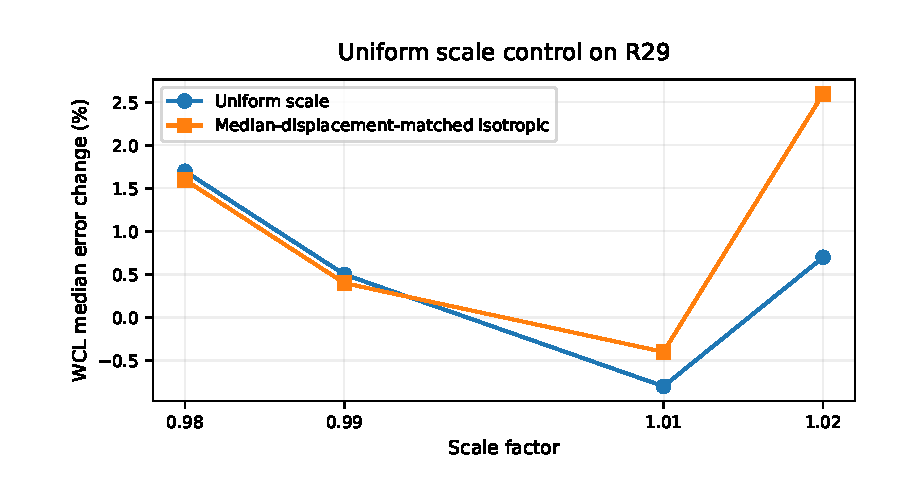
\includegraphics[width=0.88\textwidth]{FigS2_Scale_Control.pdf}
\caption{Uniform scale response compared with matched-isotropic displacement over the tested range.}
\end{figure}

\Needspace{6\baselineskip}
\subsection*{S7.1 Primary recovered-29 centroid-pivoted rotation}\label{s7.1-primary-recovered-29-centroid-pivoted-rotation}

\begin{center}\begin{minipage}{\textwidth}\centering
\captionof{table}{S7.1 Primary recovered-29 centroid-pivoted rotation}

\begin{tabular}{@{}
  >{\raggedleft\arraybackslash}p{(\columnwidth - 14\tabcolsep) * \real{0.1250}}
  >{\raggedleft\arraybackslash}p{(\columnwidth - 14\tabcolsep) * \real{0.1250}}
  >{\raggedleft\arraybackslash}p{(\columnwidth - 14\tabcolsep) * \real{0.1250}}
  >{\raggedleft\arraybackslash}p{(\columnwidth - 14\tabcolsep) * \real{0.1250}}
  >{\raggedleft\arraybackslash}p{(\columnwidth - 14\tabcolsep) * \real{0.1250}}
  >{\raggedleft\arraybackslash}p{(\columnwidth - 14\tabcolsep) * \real{0.1250}}
  >{\raggedleft\arraybackslash}p{(\columnwidth - 14\tabcolsep) * \real{0.1250}}
  >{\raggedleft\arraybackslash}p{(\columnwidth - 14\tabcolsep) * \real{0.1250}}@{}}
\toprule\noalign{}
\begin{minipage}[b]{\linewidth}\raggedleft
angle (deg)
\end{minipage} & \begin{minipage}[b]{\linewidth}\raggedleft
median displacement (m)
\end{minipage} & \begin{minipage}[b]{\linewidth}\raggedleft
WCL (\%)
\end{minipage} & \begin{minipage}[b]{\linewidth}\raggedleft
ABS (\%)
\end{minipage} & \begin{minipage}[b]{\linewidth}\raggedleft
DIFF (\%)
\end{minipage} & \begin{minipage}[b]{\linewidth}\raggedleft
Min-Max (\%)
\end{minipage} & \begin{minipage}[b]{\linewidth}\raggedleft
matched-isotropic WCL (\%)
\end{minipage} & \begin{minipage}[b]{\linewidth}\raggedleft
WCL excess (pp)
\end{minipage} \\
\midrule\noalign{}

0.5 & 43 & 3.6 & 3.2 & 1.8 & 3.2 & 0.3 & 3.3 \\
1.0 & 86 & 8.3 & 5.8 & 4.0 & 5.4 & 3.8 & 4.6 \\
2.0 & 172 & 16.2 & 12.2 & 10.9 & 12.3 & 6.0 & 10.2 \\
5.0 & 429 & 49.8 & 26.6 & 11.8 & 33.7 & 22.7 & 27.1 \\
\bottomrule
\end{tabular}
\end{minipage}\end{center}

This table is the registered R29 legacy construction: rotation about the unweighted receiver-coordinate centroid, compared with four median-displacement-matched isotropic directions. Its file-exact observation remains valid. The generalized interpretation is superseded by the pre-specified official-coordinate transfer and post-failure pivot diagnostic in Section S12; the original +27.1-point WCL excess is not represented as substrate-invariant.

\Needspace{6\baselineskip}
\subsection*{S7.2 Uniform scale}\label{s7.2-uniform-scale}
The executed scale is $\mathbf a'_i=\mathbf c_u+s(\mathbf a_i-\mathbf c_u)$, with $\mathbf c_u$ the unweighted mean of all 29 unperturbed R29 receiver coordinates and $s\in\{0.98,0.99,1.01,1.02\}$. This is not scaling about the transmitter centroid or the operational WCL centroid. For each scale, its median receiver displacement supplies the magnitude of four isotropic controls with seeds $4800+\operatorname{int}(1000s)+13r$, $r=0,1,2,3$. Map-specific intercepts are refitted after each construction.

\begin{center}\begin{minipage}{\textwidth}\centering
\captionof{table}{S7.2 Uniform scale}

\begin{tabular}{@{}
  >{\raggedleft\arraybackslash}p{(\columnwidth - 14\tabcolsep) * \real{0.1250}}
  >{\raggedleft\arraybackslash}p{(\columnwidth - 14\tabcolsep) * \real{0.1250}}
  >{\raggedleft\arraybackslash}p{(\columnwidth - 14\tabcolsep) * \real{0.1250}}
  >{\raggedleft\arraybackslash}p{(\columnwidth - 14\tabcolsep) * \real{0.1250}}
  >{\raggedleft\arraybackslash}p{(\columnwidth - 14\tabcolsep) * \real{0.1250}}
  >{\raggedleft\arraybackslash}p{(\columnwidth - 14\tabcolsep) * \real{0.1250}}
  >{\raggedleft\arraybackslash}p{(\columnwidth - 14\tabcolsep) * \real{0.1250}}
  >{\raggedleft\arraybackslash}p{(\columnwidth - 14\tabcolsep) * \real{0.1250}}@{}}
\toprule\noalign{}
\begin{minipage}[b]{\linewidth}\raggedleft
scale
\end{minipage} & \begin{minipage}[b]{\linewidth}\raggedleft
median displacement (m)
\end{minipage} & \begin{minipage}[b]{\linewidth}\raggedleft
WCL (\%)
\end{minipage} & \begin{minipage}[b]{\linewidth}\raggedleft
ABS (\%)
\end{minipage} & \begin{minipage}[b]{\linewidth}\raggedleft
DIFF (\%)
\end{minipage} & \begin{minipage}[b]{\linewidth}\raggedleft
Min-Max (\%)
\end{minipage} & \begin{minipage}[b]{\linewidth}\raggedleft
matched-isotropic WCL (\%)
\end{minipage} & \begin{minipage}[b]{\linewidth}\raggedleft
WCL excess (pp)
\end{minipage} \\
\midrule\noalign{}

0.98 & 98 & 1.7 & -0.6 & 1.8 & -1.1 & 1.6 & 0.1 \\
0.99 & 49 & 0.5 & 0.1 & 0.1 & -0.7 & 0.4 & 0.1 \\
1.01 & 49 & -0.8 & 1.7 & -2.3 & 0.5 & -0.4 & -0.4 \\
1.02 & 98 & 0.7 & 1.3 & -2.7 & 2.9 & 2.6 & -1.9 \\
\bottomrule
\end{tabular}
\end{minipage}\end{center}

\Needspace{6\baselineskip}
\subsection*{S7.3 Spatially clustered subsets}\label{s7.3-spatially-clustered-subsets}
Cluster centres are the receivers at zero-based exposure-rank indices $0,\lfloor29/3\rfloor,\lfloor2\times29/3\rfloor,28$: BS14, BS18, BS34 and BS41. For each centre, choose the $m=3$ or $7$ nearest receivers in unperturbed UTM geometry, including the centre; exact distance ties retain numeric receiver-ID order. Each subset receives two independent fixed-radius 5000-m fields with seeds $5500+m+11s+101d$, where $s=0,\ldots,3$ indexes the four centres and $d=0,1$. Thus the eight cluster cases are four subsets with two fields each, not eight independent centres. The random comparator uses four uniform $m$-subsets from Python \texttt{Random(6100+s).sample(G,m)}, $s=0,\ldots,3$, and two fields per subset with seeds $6200+s+101d$. All angles are independent uniform draws on $[0,2\pi)$ in numeric target order. Exact target lists are retained in \path{results/s4/spatial_operator_register.json}.

\begin{center}\begin{minipage}{\textwidth}\centering
\captionof{table}{S7.3 Spatially clustered subsets}

\begin{tabular}{@{}
  >{\raggedleft\arraybackslash}p{(\columnwidth - 14\tabcolsep) * \real{0.1176}}
  >{\raggedleft\arraybackslash}p{(\columnwidth - 14\tabcolsep) * \real{0.1176}}
  >{\raggedleft\arraybackslash}p{(\columnwidth - 14\tabcolsep) * \real{0.1176}}
  >{\centering\arraybackslash}p{(\columnwidth - 14\tabcolsep) * \real{0.1471}}
  >{\raggedleft\arraybackslash}p{(\columnwidth - 14\tabcolsep) * \real{0.1176}}
  >{\raggedleft\arraybackslash}p{(\columnwidth - 14\tabcolsep) * \real{0.1176}}
  >{\centering\arraybackslash}p{(\columnwidth - 14\tabcolsep) * \real{0.1471}}
  >{\raggedright\arraybackslash}p{(\columnwidth - 14\tabcolsep) * \real{0.1176}}@{}}
\toprule\noalign{}
\begin{minipage}[b]{\linewidth}\raggedleft
receivers m
\end{minipage} & \begin{minipage}[b]{\linewidth}\raggedleft
clustered WCL median (m)
\end{minipage} & \begin{minipage}[b]{\linewidth}\raggedleft
clustered change (\%)
\end{minipage} & \begin{minipage}[b]{\linewidth}\centering
clustered range (m)
\end{minipage} & \begin{minipage}[b]{\linewidth}\raggedleft
random WCL median (m)
\end{minipage} & \begin{minipage}[b]{\linewidth}\raggedleft
random change (\%)
\end{minipage} & \begin{minipage}[b]{\linewidth}\centering
random range (m)
\end{minipage} & \begin{minipage}[b]{\linewidth}\raggedright
range verdict
\end{minipage} \\
\midrule\noalign{}

3 & 739 & 23.7 & 598--901 & 600 & 0.4 & 598--602 & overlap; not separated \\
7 & 1288 & 115.5 & 598--1687 & 651 & 8.9 & 602--905 & overlap; not separated \\
\bottomrule
\end{tabular}
\end{minipage}\end{center}

Each arm uses eight draws. Complete source-file identifiers are retained in the machine-readable affine and clustering tables.

\section*{S8. Mixed-error composition and percentile reliability}\label{s8.-mixed-error-composition-and-percentile-reliability}

\begin{figure}[H]
\centering
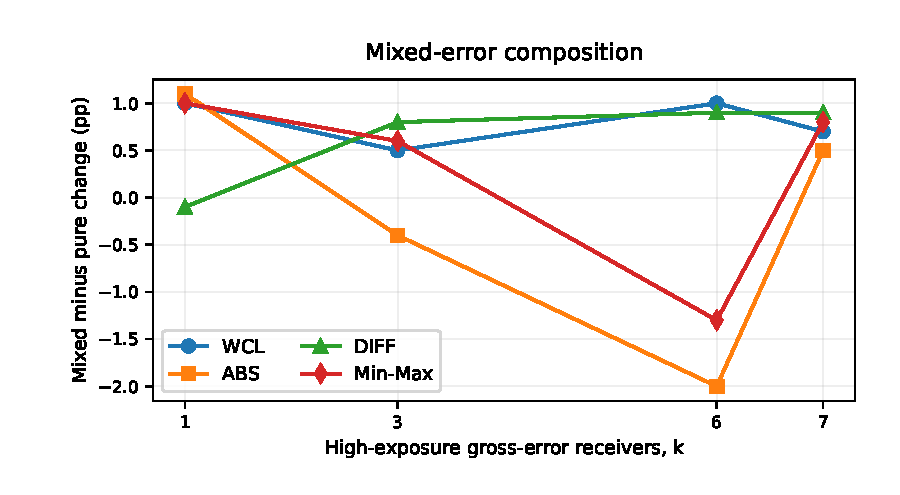
\includegraphics[width=0.88\textwidth]{FigS3_Two_Population.pdf}
\caption{Mixed-error comparison: mixed-minus-pure gaps for 20-m background jitter plus 5-km top-k errors.}
\end{figure}

\Needspace{6\baselineskip}
\subsection*{S8.1 Mixed-error comparison}\label{s8.1-two-population-mixed-error-experiment}
For draw $d=0,\ldots,3$, every R29 receiver first receives a fixed-length 20-m offset $\boldsymbol\epsilon_{id}=20(\cos\alpha_{id},\sin\alpha_{id})$, with independent uniform angles from NumPy \texttt{default\_rng(4400+d)}. The 20 m is a radius, not a Gaussian standard deviation or Rayleigh scale. In the mixed arm, top-$k$ receivers ($k=1,3,6,7$) additionally receive $\boldsymbol\eta_{ikd}=5000(\cos\theta_{ikd},\sin\theta_{ikd})$, from seed $8800+k+101d$. Pure and mixed arms share this exact gross-error field and the evaluation population; the background field is shared across $k$ at the same $d$. Offsets add vectorially, so the mixed target displacement need not be exactly 5000 or 5020 m. Each resulting map is separately recalibrated. The reported gap subtracts the two across-field central error summaries; it is not an individual-message composition law.

The reported gap is the mixed-error minus pure top-$k$ median summary in percentage points against the same reference, using four registered direction realizations. Gaps within about two points describe this 20-m-plus-5-km regime, not linear superposition or an individual-message composition law.

\begin{center}\begin{minipage}{\textwidth}\centering
\captionof{table}{S8.1 Mixed-error comparison}

\begin{tabular}{@{}
  >{\raggedleft\arraybackslash}p{(\columnwidth - 12\tabcolsep) * \real{0.14285}}
  >{\raggedleft\arraybackslash}p{(\columnwidth - 12\tabcolsep) * \real{0.14285}}
  >{\raggedleft\arraybackslash}p{(\columnwidth - 12\tabcolsep) * \real{0.14285}}
  >{\raggedleft\arraybackslash}p{(\columnwidth - 12\tabcolsep) * \real{0.14285}}
  >{\raggedleft\arraybackslash}p{(\columnwidth - 12\tabcolsep) * \real{0.14285}}
  >{\raggedleft\arraybackslash}p{(\columnwidth - 12\tabcolsep) * \real{0.14285}}
  >{\raggedleft\arraybackslash}p{(\columnwidth - 12\tabcolsep) * \real{0.14285}}@{}}
\toprule\noalign{}
\begin{minipage}[b]{\linewidth}\raggedleft
k
\end{minipage} & \begin{minipage}[b]{\linewidth}\raggedleft
mixed-error WCL (\%)
\end{minipage} & \begin{minipage}[b]{\linewidth}\raggedleft
pure top-k WCL (\%)
\end{minipage} & \begin{minipage}[b]{\linewidth}\raggedleft
WCL gap (pp)
\end{minipage} & \begin{minipage}[b]{\linewidth}\raggedleft
ABS gap (pp)
\end{minipage} & \begin{minipage}[b]{\linewidth}\raggedleft
DIFF gap (pp)
\end{minipage} & \begin{minipage}[b]{\linewidth}\raggedleft
Min-Max gap (pp)
\end{minipage} \\
\midrule\noalign{}

1 & 4.5 & 3.5 & 1.0 & 1.1 & -0.1 & 1.0 \\
3 & 27.9 & 27.4 & 0.5 & -0.4 & 0.8 & 0.6 \\
6 & 51.0 & 50.0 & 1.0 & -2.0 & 0.9 & -1.3 \\
7 & 226.6 & 225.8 & 0.7 & 0.5 & 0.9 & 0.8 \\
\bottomrule
\end{tabular}
\end{minipage}\end{center}

The mixed-error comparisons use four registered direction replicates on the fixed evaluation population. The reported gaps are descriptive contrasts of replicate-level summaries; four perturbation replicates are not treated as an inferential sample size.

\Needspace{6\baselineskip}
\subsection*{S8.2 WCL percentile profile}\label{s8.2-wcl-percentile-profile}

\begin{center}\begin{minipage}{\textwidth}\centering
\captionof{table}{S8.2 WCL percentile profile}

\begin{tabular}{@{}lrrrrr@{}}
\toprule\noalign{}
condition & P50 (m) & P75 (m) & P90 (m) & P95 (m) & pooled evaluations \\
\midrule\noalign{}

reference & 598 & 1070 & 1652 & 2012 & 2498 \\
24\% at 5 km & 775 & 1249 & 1751 & 2237 & 9992 \\
100\% at 5 km & 2730 & 3893 & 4795 & 5091 & 9992 \\
top-six at 5 km & 887 & 2287 & 3520 & 4097 & 9992 \\
top-seven at 5 km & 1960 & 3122 & 4048 & 4409 & 9992 \\
\bottomrule
\end{tabular}
\end{minipage}\end{center}

The top-six-to-top-seven increments are 1,073 m at P50, 528 m at P90 and 312 m at P95. These marginal quantiles do not identify harmed-message subgroups or exclude a newly affected minority. For each perturbed row, 9,992 equals four direction replicates multiplied by the same 2,498 unique evaluation messages. These are repeated message--condition evaluations, not 9,992 independent messages. The percentile table is a descriptive mixture over the registered directions; no confidence interval or hypothesis test in this paper uses 9,992 as an independent sample size. The complete source mapping is supplied in \texttt{paperb\_twopop.csv} and \texttt{paperb\_tails.csv}.

\section*{S9. DIFF pair-admission repair}\label{s9.-diff-pair-admission-repair}

The intended DIFF contract drops the 3-dB pair threshold when fewer than two pairs survive. The audit found invocation in 1.00\% of reference messages and up to 11.17\% in a severe-corruption condition. The entire DIFF-bearing suite was regenerated. Across 2,127 compared non-DIFF scalar fields, WCL, ABS, and Min-Max had zero mismatches. Repaired DIFF values supersede the historical values.

Key changes: reference 966-\textgreater964 m; full 5-km corruption +95.4\%-\textgreater+89.2\%; full 10-km corruption +266.3\%-\textgreater+242.9\%; 5-km top-six-\textgreater top-seven +13.5\%-\textgreater+53.7\% became +13.4\%-\textgreater+48.8\%. Every manuscript-level conclusion survived.

\section*{S10. Provenance and reproduction access}\label{s10.-provenance-and-reproducibility}
The accompanying computational evidence package contains the pair-fallback-audited canonical harness, exact evaluator and projected maps; calibration/evaluation source-row manifests; retained raw logs and author arrays; perturbation specifications; ranges and figure data; and a read-only checksum verifier. Source CSV observations retain their original publisher terms and are obtained separately using the pinned version/hash. The package README gives verification and reproduction commands. \path{results/rc5/CURRENT_ENVIRONMENT.json} records the environment tested for reporting recovery and rendering; it is not presented as the missing historical dependency freeze.

Original author-run archives remain unchanged in the full repository candidate. Reporting-recovery outputs and bootstrap-verification derivatives are separately labelled. The common-27 maps retain identical ordered evaluation IDs. A code/version manifest distinguishes the present DIFF fallback implementation from historical outputs, which are not used as current numerical authority. MIT applies to project code; CC BY 4.0 applies to author-created documentation and derived non-code artifacts, with third-party terms preserved.

\noindent The current input-provenance entry point is \texttt{coordinate\_provenance/README.md}; S15 describes the attributed sources and the frozen-map verification/rebuild routes. The current claim index is \path{results/CLAIM_TO_ARTIFACT_SENSORS_S6.csv}; \path{results/CLAIM_TO_ARTIFACT_RC8.csv} is the unchanged baseline index. Earlier governance and source logs remain immutable historical records; their legacy labels (for example, ``true map'' or ``repair'') do not override the qualifications in this revision. Source attribution and historical records are not claims that another manuscript has been published.

\section*{S11. Statistical interpretation and precision checks}\label{s11.-statistical-interpretation-and-precision-checks}

\Needspace{6\baselineskip}
\subsection*{S11.1 Estimands and replicate hierarchy}

For each method and perturbation replicate, the elementary outcome is message-level localization error and the replicate summary is its median over the fixed evaluation messages. Multi-replicate condition summaries use the median of those replicate-level medians. Receiver-choice and direction min--max values are therefore perturbation-design sensitivity ranges, not confidence intervals. Evaluation/calibration redraw diagnostics, perturbation-replicate dispersion, and message-level event proportions are kept as distinct uncertainty objects. No post-hoc $p$-value or multiplicity screen is introduced in B9B.

\Needspace{6\baselineskip}
\subsection*{S11.2 Top-six to top-seven effect-size persistence}

\begin{center}\begin{minipage}{\textwidth}\centering
\captionof{table}{S11.2 Top-six to top-seven effect-size persistence}

\begin{tabular}{@{}llrrrr@{}}
\toprule\noalign{}
setting & method & k=6 (\%) & k=7 (\%) & jump (pp) & perturbation draws \\
\midrule\noalign{}

5 km, max\_gws=10 & WCL & 49.5 & 233.4 & 183.9 & 8 \\
5 km, max\_gws=10 & ABS & 38.2 & 65.0 & 26.8 & 8 \\
5 km, max\_gws=10 & DIFF & 13.4 & 48.8 & 35.4 & 8 \\
5 km, max\_gws=10 & Min-Max & 98.0 & 243.3 & 145.3 & 8 \\
1 km, max\_gws=10 & WCL & 25.5 & 47.3 & 21.8 & 4 \\
1 km, max\_gws=10 & ABS & 20.3 & 39.5 & 19.2 & 4 \\
1 km, max\_gws=10 & DIFF & 27.0 & 45.6 & 18.6 & 4 \\
1 km, max\_gws=10 & Min-Max & 26.8 & 48.0 & 21.2 & 4 \\
5 km, max\_gws=5 & WCL & 60.9 & 251.1 & 190.2 & 4 \\
5 km, max\_gws=5 & ABS & 36.7 & 63.6 & 26.9 & 4 \\
5 km, max\_gws=5 & DIFF & 17.2 & 49.6 & 32.4 & 4 \\
5 km, max\_gws=5 & Min-Max & 103.5 & 277.0 & 173.5 & 4 \\
\bottomrule
\end{tabular}
\end{minipage}\end{center}

All twelve jumps are positive across three apparatus settings. Their amplitudes vary strongly by architecture and setting, so this table is evidence for boundary-location persistence, not for a universal cliff magnitude. The four- and eight-direction rows remain small perturbation-replicate sets; effect sizes and registered ranges, rather than replicate-level $p$-values, carry the claim.

\Needspace{6\baselineskip}
\subsection*{S11.3 Exhaustion-increment finite-message precision}

\begingroup\footnotesize
\begin{center}\begin{minipage}{\textwidth}\centering
\captionof{table}{S11.3 Exhaustion-increment finite-message precision}

\begin{tabular}{@{}p{0.25\columnwidth}rrrrr@{}}
\toprule\noalign{}
deployment / window & $N$ & newly exhausted & $\Delta C(7)$ (pp) & Wilson lo & Wilson hi \\
\midrule\noalign{}

Antwerp, max\_gws=10 & 2498 & 355 & 14.2114 & 12.8970 & 15.6356 \\
Antwerp, max\_gws=5 & 2498 & 355 & 14.2114 & 12.8970 & 15.6356 \\
Sigfox urban, max\_gws=10 & 13163 & 6 & 0.0456 & 0.0209 & 0.0994 \\
Sigfox rural, max\_gws=10 & 23467 & 2822 & 12.0254 & 11.6155 & 12.4478 \\
\bottomrule
\end{tabular}
\end{minipage}\end{center}
\endgroup

The interval is applied to the Bernoulli indicator that a message is newly exhausted when moving from $T_6$ to $T_7$. Because $T_6\subset T_7$, the increment is an observed nested-message proportion rather than a difference of two independent proportions. The Wilson intervals are binomial-reference orientation checks under an iid-message approximation; they neither establish message independence, correct campaign-level temporal/spatial dependence, nor convert the Sigfox controls into localization experiments.

\Needspace{6\baselineskip}
\subsection*{S11.4 Scope of negative and bounded results}

The approximately matched exposure bins contain varied outcomes while exact exposure, receiver composition/count and directions change together; they do not isolate co-occurrence or refute every function of exact exposure. The clustered experiment remains bounded by overlapping eight-draw ranges; no power or separation claim is inferred from those draws. The percentile falsifier pools four registered direction replicates over the same 2,498 messages, so 9,992 denotes repeated evaluations rather than independent observations. Sections S12--S13 add pre-specified reference-substrate, exponent, and dependence safeguards. Failed transfer criteria remain failed; explanatory diagnostics do not replace confirmatory tests or introduce post-hoc significance thresholds.


\section*{S12. Reference-substrate, exact-seven, exponent, and rotation safeguards}\label{s12.-reference-substrate-exact-seven-exponent-and-rotation-safeguards}

\Needspace{6\baselineskip}
\subsection*{S12.1 Frozen status and substrate hierarchy}

Internal labels distinguish the pre-safeguard scientific package (B9B) from the reference/exponent/dependence safeguard stage (B9C). G4 denotes the legacy rotation-transfer criterion, G5 the propagation-exponent criterion, and G6 the spatial-cell criterion. These are project experiment labels, not journal review rounds.

The B9C protocol was frozen after the B9B scientific package and before the official-coordinate outputs were inspected. R29 remains primary. O32$-$71 uses catalogue coordinates with BS71 excluded; R27/O27 holds identities and ordered messages fixed, with BS71 at the R29 coordinate in both arms. O27 is therefore a mixed-reference construction. The published/substituted 33-receiver arms test BS71 sensitivity, not independently surveyed truth. Table~\ref{tab:s-map-parents} identifies all parent maps. These clarifications describe the original runner and do not change a protocol, input, result or failed criterion.

\begin{center}\begin{minipage}{\textwidth}\centering
\captionof{table}{S12.1 Frozen status and substrate hierarchy}

\begin{tabular}{@{}lrrrr@{}}
\toprule
substrate / 10-km condition & WCL (\%) & ABS (\%) & DIFF (\%) & Min-Max (\%) \\
\midrule

R29, one receiver & 0.1 & 0.6 & -0.8 & 0.1 \\
R29, all receivers & 845.2 & 369.8 & 242.9 & 582.9 \\
O32$-$71, one receiver & 0.5 & -0.1 & -3.4 & 6.1 \\
O32$-$71, all receivers & 895.3 & 399.4 & 188.3 & 581.5 \\
\bottomrule
\end{tabular}
\end{minipage}\end{center}

The sparse--dense transfer criterion passes: on O32$-$71, every one-receiver absolute effect is no greater than 10\%, every full-roster effect exceeds +100\%, and each full-roster effect exceeds its sparse counterpart.

\Needspace{6\baselineskip}
\subsection*{S12.2 Exact-seven completion across eight roster constructions}

The legacy fraction generator used roster-dependent quarter counts, so B9C explicitly executed exactly seven corrupted receivers under eight recovered/official roster constructions, eight registered draws per cell.

\begin{center}\begin{minipage}{\textwidth}\centering
\captionof{table}{S12.2 Exact-seven completion across eight roster constructions}

\begin{tabular}{@{}rlrr@{}}
\toprule
$D$ (m) & method & minimum effect (\%) & maximum effect (\%) \\
\midrule

1000 & ABS & 3.0 & 10.3 \\
1000 & DIFF & 3.1 & 19.6 \\
1000 & Min-Max & 4.9 & 12.2 \\
1000 & WCL & 3.3 & 12.5 \\
\addlinespace[4pt]\midrule
10000 & ABS & 9.1 & 18.8 \\
10000 & DIFF & -26.3 & -1.7 \\
10000 & Min-Max & 23.9 & 58.8 \\
10000 & WCL & 10.0 & 24.6 \\
\bottomrule
\end{tabular}
\end{minipage}\end{center}

At 10 km, WCL, ABS, and Min-Max are worse than their roster-specific references in every exact-seven arm, whereas DIFF's central median improves in all eight. The result is retained as architecture- and substrate-conditioned non-monotonicity, not as evidence that coordinate corruption is beneficial.

\Needspace{6\baselineskip}
\subsection*{S12.3 Exposure-boundary transfer at 5 km}

\begin{center}\begin{minipage}{\textwidth}\centering
\captionof{table}{S12.3 Exposure-boundary transfer at 5 km}

\begin{tabular}{@{}lrrrr@{}}
\toprule
coordinate configuration & WCL jump (pp) & ABS jump (pp) & DIFF jump (pp) & Min-Max jump (pp) \\
\midrule

R29 & 183.9 & 26.8 & 35.4 & 145.3 \\
O32$-$71 & 111.3 & 53.3 & 36.9 & 93.3 \\
R27 common roster & 188.4 & 28.6 & 33.3 & 145.3 \\
O27 common roster & 127.0 & 59.2 & 42.8 & 118.5 \\
\bottomrule
\end{tabular}
\end{minipage}\end{center}

All four $k=6\rightarrow7$ jumps are positive in the standard ten-receiver window. In native official-33 with BS71 substituted by its R29 coordinate, changing the message window moves BS 10 from rank seven to rank six. The same 335 messages become newly exhausted when BS 10 enters: at $k=7$ under the ten-receiver window and at $k=6$ under the five-receiver window. Among the two adjacent increases from $k=5$ to 6 and from $k=6$ to 7, WCL, ABS, and DIFF move the larger increase with that support-loss event; Min-Max retains the larger increase from six to seven. The result supports a participation-set boundary rather than a universal integer threshold.

\Needspace{6\baselineskip}
\noindent\textbf{Executed O33 window control.} Both runs use \path{maps/official33_repaired71.json}, the inherited filename for O33-substituted, and the same ordered 2495-message population. At cap ten, the entering receivers at $k=6,7$ are BS9 and BS10, with 37 and 335 newly exhausted messages. At cap five, they are BS10 and BS32, with 335 and 107. The saved selected-identity record reproduces equality of the two 335-message sets, not merely equality of their counts. Its identifiers are retained working-message indices, not original CSV row indices; \path{results/s4/o33_identity_equality.json} preserves the two equal lists and that distinction.

\begin{center}\begin{minipage}{\textwidth}\centering\small
\captionof{table}{O33-substituted top-ranked corruption at 5 km: absolute median errors and increments in metres. Values are the retained whole-metre log summaries; increments are differences at that precision, not recovered full-precision estimates. Each condition has eight fields for cap ten and four for cap five. The corresponding percentage-point increments and identity counts appear in the main article and the machine-readable reporting tables.}\label{tab:so33window}
\begin{tabular}{rlrrrrr}
\toprule Cap & Method & $M_5$ & $M_6$ & $M_7$ & $M_6-M_5$ & $M_7-M_6$\\\midrule
10 & WCL & 700 & 725 & 1476 & +25 & +751\\
10 & ABS & 551 & 567 & 897 & +16 & +330\\
10 & DIFF & 854 & 862 & 1273 & +8 & +411\\
10 & Min-Max & 652 & 725 & 1227 & +73 & +502\\
5 & WCL & 677 & 1255 & 1568 & +578 & +313\\
5 & ABS & 597 & 827 & 934 & +230 & +107\\
5 & DIFF & 901 & 1235 & 1274 & +334 & +39\\
5 & Min-Max & 723 & 976 & 1271 & +253 & +295\\
\bottomrule
\end{tabular}
\end{minipage}\end{center}


The method-specific percentage-point increments are displayed in the main window-control table and in the machine-readable reporting table. Each percentage uses that method and window's reference; increments subtract retained one-decimal summaries and are not full-precision paired effects. Cap ten uses eight direction fields per condition, cap five four. Independent uniform angles use seed $8800+k+101r$ in numeric target order. Changing $k$ changes seeds; changing cap can change target membership. Thus the migration is not an isolated exhaustion-only intervention. Sources are the \path{O33R71_N4P7_D5000_W10.txt} and \path{O33R71_N4P7_D5000_W5.txt} logs/commands under \path{results/rc5/official_core_logs/}, with exact source rows and the adjacent percentage/count table in \path{results/s4/}.
\subsection*{S12.4 Propagation-exponent sensitivity}

\begin{center}\begin{minipage}{\textwidth}\centering
\captionof{table}{S12.4 Propagation-exponent sensitivity}

\begin{tabular}{@{}llrrr@{}}
\toprule
substrate & contrast / method & $n=3.5$ & $n=4.7$ & $n=6.0$ \\
\midrule

R29 & dense minus sparse, WCL (pp) & 841.8 & 845.1 & 856.8 \\
R29 & top-seven minus top-six, WCL (pp) & 195.0 & 183.9 & 190.7 \\
R29 & legacy rotation minus isotropic, WCL (pp) & 27.4 & 29.9 & 25.8 \\
R29 & pivot-controlled rotation contrast, WCL (pp) & 6.3 & 8.7 & 7.5 \\
O32$-$71 & dense minus sparse, WCL (pp) & 944.0 & 894.8 & 877.0 \\
O32$-$71 & top-seven minus top-six, WCL (pp) & 109.3 & 111.3 & 118.7 \\
O32$-$71 & legacy rotation minus isotropic, WCL (pp) & -1.6 & -3.9 & -7.5 \\
O32$-$71 & pivot-controlled rotation contrast, WCL (pp) & 8.0 & 8.3 & 8.3 \\
\bottomrule
\end{tabular}
\end{minipage}\end{center}

For both substrates, the dense-minus-sparse and top-seven-minus-top-six signs are stable for all four architectures. The legacy rotation sign is stable for four methods on R29 and three on O32$-$71; the WCL sign reversal across substrates is itself stable. The pivot-controlled exact-magnitude rotation residual is positive for WCL on both substrates throughout the exponent range. The frozen exponent criterion passes. This is sign stability of the reported central contrasts, not separation from all sampled directions; S14 and the evidence register expose all four methods and their retained ranges.

\Needspace{6\baselineskip}
\subsection*{S12.5 Rotation-transfer failure and post-failure geometric diagnostic}

\begin{center}\begin{minipage}{\textwidth}\centering
\captionof{table}{S12.5 Rotation-transfer failure and post-failure geometric diagnostic}

\begin{tabular}{@{}llrrr@{}}
\toprule
construction & substrate & rotation (\%) & isotropic (\%) & excess (pp) \\
\midrule

legacy unweighted-centroid & R29 & 49.8 & 19.9 & 29.9 \\
legacy unweighted-centroid & O32$-$71 & 11.0 & 14.9 & -3.9 \\
operational-centroid, exact magnitudes & R29 & 12.4 & 3.7 & 8.7 \\
operational-centroid, exact magnitudes & O32$-$71 & 5.6 & -2.7 & 8.3 \\
\bottomrule
\end{tabular}
\end{minipage}\end{center}

The legacy transfer criterion required a positive O32$-$71 WCL rotation-minus-isotropic excess and therefore fails. Rotation about the unweighted centroid $c_u$ decomposes exactly as
\begin{equation}\label{eq:s-display-1}
c_u+R(x-c_u)=c_o+R(x-c_o)+(R-I)(c_o-c_u),
\end{equation}
where $c_o$ is the corrected-WCL operational centroid. On R29, the $+5^{\circ}$ construction induces a 293.0-m coherent shift at $326.7^{\circ}$, aligned with the adverse coherent-angle sector; on O32$-$71 the shift is 137.5 m at $22.5^{\circ}$. The operational-centroid/exact-magnitude rows are post-failure explanatory diagnostics. They give a positive contrast to the median of the specified controls, not a direction-uniform residual penalty, and do not retrospectively pass the legacy transfer criterion. The comparator values and ranges are reported in S14; on R29 the rotation lies inside the sampled range. The matched refit/frozen comparisons in S12.7 support both signs of the WCL refitting intervention within the tested constructions, not an established radial-versus-bearing rule.



\Needspace{6\baselineskip}
\subsection*{S12.6 Operational pivot and common-roster rotation control}

On each unperturbed map, intercepts are fitted on the frozen calibration split. For each evaluation message with at least three mapped and calibrated receptions, take up to ten strongest raw-RSSI receivers, denoted $H_q$, and form
\begin{equation}\label{eq:s-display-2}
\alpha_{qi}=\frac{10^{(\mathrm{RSSI}_{qi}-A_{0,i})/10}}
 {\sum_{j\in H_q}10^{(\mathrm{RSSI}_{qj}-A_{0,j})/10}},\qquad
 c_o=\frac{1}{|\mathcal Q|}\sum_{q\in\mathcal Q}\sum_{i\in H_q}\alpha_{qi}a_i.
\end{equation}
Here $\mathcal Q$ contains the eligible messages in that named evaluation population. No evaluation transmitter coordinate or localization-error outcome enters this pivot calculation; reference-map intercepts retain their calibration-data dependence. The pivot is computed on the reference map for the specified exponent and retained during the controlled perturbation. It characterizes this corpus and WCL weighting, not a surveyed physical center. Re-expressing a rotation about $c_o$ gives an exact coordinate identity but does not make median localization errors additive.

The same-roster diagnostic below holds the 27 receiver identities and ordered 2,498-message population fixed. Both maps are rotated about their own unweighted coordinate centroids; the median-displacement-matched comparator uses eight directions. The map-specific pivot and displacement profiles therefore remain part of the assignment intervention. The table does not claim a fixed-pivot-only or bearing-only causal effect.

\begin{center}\begin{minipage}{\textwidth}\centering
\captionof{table}{S12.6 Operational pivot and common-roster rotation control}

\begin{tabular}{@{}llrrrr@{}}
\toprule
substrate & method & $+5^{\circ}$ (\%) & $-5^{\circ}$ (\%) & isotropic (\%) & $+5^{\circ}$ excess (pp) \\
\midrule

R27 & WCL & 41.09 & -12.56 & 15.87 & 25.22 \\
R27 & ABS & 21.79 & -19.71 & 0.10 & 21.69 \\
R27 & DIFF & 10.44 & -17.26 & 17.42 & -6.98 \\
R27 & Min-Max & 24.00 & -9.04 & -0.17 & 24.17 \\
O27 & WCL & 4.30 & 4.54 & -3.64 & 7.94 \\
O27 & ABS & -1.47 & 4.76 & -4.66 & 3.19 \\
O27 & DIFF & 1.76 & -2.28 & 7.63 & -5.87 \\
O27 & Min-Max & 4.85 & 2.11 & -2.57 & 7.42 \\
\bottomrule
\end{tabular}
\end{minipage}\end{center}

In this R27/O27 control, BS71 has the recovered coordinate in both reference arms; O27's remaining entries are catalogue-derived. Each rotation/translation field is then constructed from its named reference and pivot. The positive WCL central contrasts show different amplitudes within this mixed-reference common-roster design, not an assignment-only sign reversal or a test of the catalogue BS71 value. These populations also differ from the benchmark audit's historical common-27 population.

Source: \path{results/b9c_author_remaining/rotation_cause_results.csv}. These are post-failure diagnostics reproduced on the author's machine, not new confirmatory tests; G4 remains failed.

\Needspace{14\baselineskip}
\subsection*{S12.7 Matched rotation refit/frozen comparisons}\label{s12.7-rotation-refitting}
These six retained post-failure WCL comparisons use $n=4.7$, at most ten strongest mapped-and-calibrated receptions, and the same 2,498 messages within each pair. The two native configurations have different message identities despite equal counts. Each pair holds the rotated coordinates, target set, angle, pivot, raw RSSI and evaluation population fixed. Refitted intercepts use the unchanged calibration records on that rotated map; frozen intercepts retain their reference-map fit. The reference operational pivot $c_o$ is fixed before either arm, as defined in S12.6. Each row is a message median for one deterministic rotation, not a median across eight fields.

\begin{center}\begin{minipage}{\textwidth}\centering\small
\captionof{table}{Six existing rotation refit/frozen pairs. Differences use full-precision medians before rounding; positive harms: refitting increases median error.}\label{tab:s-rotation-refit-frozen}
\begin{tabular}{@{}llrrrr@{}}
\toprule
Reference & Pivot / angle & Refit (m) & Frozen (m) & $\Delta$ (m) & $\Delta$ (pp) \\
\midrule
R29 & $c_u,+5^\circ$ & 895.26 & 866.39 & +28.88 & +4.83 \\
R29 & $c_u,-5^\circ$ & 548.11 & 609.36 & -61.25 & -10.25 \\
R29 & $c_o,+5^\circ$ & 671.56 & 679.92 & -8.36 & -1.40 \\
O32$-$71 & $c_u,+5^\circ$ & 659.11 & 616.29 & +42.82 & +7.21 \\
O32$-$71 & $c_u,-5^\circ$ & 598.96 & 606.35 & -7.39 & -1.25 \\
O32$-$71 & $c_o,+5^\circ$ & 627.08 & 607.31 & +19.77 & +3.33 \\

\bottomrule
\end{tabular}
\end{minipage}\end{center}
Here $\Delta=M_{\mathrm{refit}}-M_{\mathrm{frozen}}$ and the percentage-point contrast is $100\Delta/M_0$, with reference median $M_0=597.672677$ m on R29 and $593.742522$ m on O32$-$71. Both unperturbed refit/frozen arms return their corresponding $M_0$. The within-pair intervention has both signs across these constructions; it is not a universal mediation law, an exponent sweep or a replacement for the failed rotation-transfer criterion.

Sources: \path{author_remaining/rotation/a0_rotation_diagnostic.csv} and \path{a0_rotation_cases.json} in that same directory. The original producer exported 16 scalar case records, not the frozen-arm per-message error arrays. The displayed six-pair register agrees with those saved cases; this is scalar consistency, not newly rederived message errors. The original producer is supplied in the retained replay ZIP; \path{results/rc8/REPORTING_SOURCE_BINDING.json} records the precise source identities. G4 remains failed.

\section*{S13. Dependence-aware precision and spatial concentration}\label{s13.-dependence-aware-precision-and-spatial-concentration}

\Needspace{6\baselineskip}
\subsection*{S13.1 Spatial-cell cluster bootstrap}

For each method, let $e_{qkr}$ be message $q$'s error in condition $k\in\{6,7\}$ and registered direction realization $r$. Define
\begin{equation}\label{eq:s-display-3}
u_{qk}=\operatorname{median}_{r=0,\ldots,7}e_{qkr},\qquad
 T=\operatorname{median}_q u_{q7}-\operatorname{median}_q u_{q6}.
\end{equation}
On R29 WCL, the primary median-across-realizations top-seven-minus-top-six contrast is approximately 1,099 m, while the direction-first statistic $T$ is 1,411.92 m. The order of medians is not interchangeable. Thus $T$ is a difference of two medians of direction-summarized errors, not the median of paired differences and not the primary median-of-replicate-medians contrast. Resampling preserves each message's two condition values together. The seeds are $8800+k+101r$, so the two conditions have eight registered realizations but not identical direction vectors.

For cell width $h$, projected coordinates $(x_q,y_q)$ receive label $(\lfloor x_q/h\rfloor,\lfloor y_q/h\rfloor)$, fixing the grid origin at zero in the dataset's projected coordinate system. Occupied-cell labels are sorted. Each of 2,000 replicates samples the original number of cells with replacement, concatenates all messages in the sampled cells, and recomputes $T$ and the newly-exhausted-message proportion. Replicate message counts may vary because cell sizes differ. The spatial seed is $960000+10000s+h$, where $s=0$ for R29 and $s=1$ for O32$-$71. Intervals below are percentile cluster-bootstrap intervals; they characterize sensitivity to the observed spatial-cell composition, not a superpopulation confidence guarantee.

\begin{longtable}[]{@{}lrlrrr@{}}
\caption{S13.1 Spatial-cell cluster bootstrap}\\
\toprule
substrate & cell width (m) & estimand & point & 95\% lo & 95\% hi \\
\midrule
\endhead
\bottomrule
\endlastfoot
R29 & 500 & WCL (m) & 1411.92 & -27.13 & 2417.57 \\
R29 & 500 & ABS (m) & 171.45 & -42.04 & 421.51 \\
R29 & 500 & DIFF (m) & 351.88 & -45.44 & 741.58 \\
R29 & 500 & Min-Max (m) & 774.49 & 7.47 & 1757.48 \\
R29 & 500 & exhaustion (pp) & 14.21 & 0.00 & 31.14 \\
R29 & 1000 & WCL (m) & 1411.92 & -24.75 & 2486.18 \\
R29 & 1000 & ABS (m) & 171.45 & -38.25 & 463.19 \\
R29 & 1000 & DIFF (m) & 351.88 & -51.85 & 798.65 \\
R29 & 1000 & Min-Max (m) & 774.49 & -10.28 & 1832.35 \\
R29 & 1000 & exhaustion (pp) & 14.21 & 0.00 & 33.76 \\
R29 & 2000 & WCL (m) & 1411.92 & -42.44 & 2421.43 \\
R29 & 2000 & ABS (m) & 171.45 & -51.28 & 465.52 \\
R29 & 2000 & DIFF (m) & 351.88 & -69.91 & 837.05 \\
R29 & 2000 & Min-Max (m) & 774.49 & 2.20 & 1804.86 \\
R29 & 2000 & exhaustion (pp) & 14.21 & 0.00 & 33.84 \\
O32$-$71 & 500 & WCL (m) & 687.01 & -4.21 & 1951.39 \\
O32$-$71 & 500 & ABS (m) & 276.74 & -22.29 & 700.41 \\
O32$-$71 & 500 & DIFF (m) & 399.15 & 2.84 & 1110.12 \\
O32$-$71 & 500 & Min-Max (m) & 461.22 & -0.99 & 1384.83 \\
O32$-$71 & 500 & exhaustion (pp) & 13.09 & 0.00 & 29.36 \\
O32$-$71 & 1000 & WCL (m) & 687.01 & -5.46 & 1971.74 \\
O32$-$71 & 1000 & ABS (m) & 276.74 & -20.65 & 733.69 \\
O32$-$71 & 1000 & DIFF (m) & 399.15 & 3.67 & 1189.76 \\
O32$-$71 & 1000 & Min-Max (m) & 461.22 & -4.98 & 1466.57 \\
O32$-$71 & 1000 & exhaustion (pp) & 13.09 & 0.00 & 30.89 \\
O32$-$71 & 2000 & WCL (m) & 687.01 & -9.66 & 1985.48 \\
O32$-$71 & 2000 & ABS (m) & 276.74 & -28.97 & 745.56 \\
O32$-$71 & 2000 & DIFF (m) & 399.15 & -3.67 & 1215.51 \\
O32$-$71 & 2000 & Min-Max (m) & 461.22 & 1.29 & 1513.86 \\
O32$-$71 & 2000 & exhaustion (pp) & 13.09 & 0.00 & 31.91 \\
\end{longtable}

Every method has a positive point estimate at every width and exhaustion remains positive, but the 1-km WCL intervals include zero on both substrates. The frozen spatial-cell criterion therefore fails.

\Needspace{6\baselineskip}
\subsection*{S13.2 Cause of the spatial failure}

\begin{center}\begin{minipage}{\textwidth}\centering
\captionof{table}{S13.2 Cause of the spatial failure}

\begin{tabular}{@{}lrrrrr@{}}
\toprule
substrate & width (m) & occupied cells & newly exhausted & active cells & largest-cell share \\
\midrule

R29 & 500 & 106 & 355 & 2 & 99.72\% \\
R29 & 1000 & 39 & 355 & 2 & 99.72\% \\
R29 & 2000 & 12 & 355 & 1 & 100.00\% \\
O32$-$71 & 500 & 106 & 327 & 2 & 99.69\% \\
O32$-$71 & 1000 & 41 & 327 & 2 & 99.69\% \\
O32$-$71 & 2000 & 14 & 327 & 1 & 100.00\% \\
\bottomrule
\end{tabular}
\end{minipage}\end{center}

At 500 m and 1 km, 354/355 newly exhausted R29 messages and 326/327 O32$-$71 messages occupy one dominant cell; at 2 km all newly exhausted messages occupy one cell. At 500 m and 1 km, omitting the dominant cell removes almost all newly exhausted messages, not necessarily every such message; at 2 km, all newly exhausted messages occupy one cell. This concentration supports a geographically conditional interpretation. It does not prove that exhaustion alone causes the localization shift.

\Needspace{6\baselineskip}
\subsection*{S13.3 Temporal-block sensitivity}

Source \texttt{RX Time} values are parsed in UTC. A timestamp with Unix epoch seconds $t_q$ receives label $\lfloor t_q/(60b)\rfloor$ for block width $b\in\{5,15,30\}$ minutes. Sorted occupied blocks are resampled using the same whole-block procedure and statistic as in S13.1, with seed $970000+10000s+b$. These are time blocks, not independently identified trajectories.

\begin{longtable}[]{@{}lrlrrr@{}}
\caption{S13.3 Temporal-block sensitivity}\\
\toprule
substrate & block (min) & estimand & point & 95\% lo & 95\% hi \\
\midrule
\endhead
\bottomrule
\endlastfoot
R29 & 5 & WCL (m) & 1411.92 & 1207.99 & 1572.05 \\
R29 & 5 & ABS (m) & 171.45 & 140.51 & 206.38 \\
R29 & 5 & DIFF (m) & 351.88 & 302.67 & 412.26 \\
R29 & 5 & Min-Max (m) & 774.49 & 694.32 & 876.25 \\
R29 & 5 & exhaustion (pp) & 14.21 & 12.69 & 15.63 \\
R29 & 15 & WCL (m) & 1411.92 & 1185.85 & 1592.25 \\
R29 & 15 & ABS (m) & 171.45 & 138.37 & 209.02 \\
R29 & 15 & DIFF (m) & 351.88 & 298.66 & 412.33 \\
R29 & 15 & Min-Max (m) & 774.49 & 683.76 & 890.72 \\
R29 & 15 & exhaustion (pp) & 14.21 & 12.72 & 15.74 \\
R29 & 30 & WCL (m) & 1411.92 & 1167.68 & 1590.22 \\
R29 & 30 & ABS (m) & 171.45 & 139.84 & 208.88 \\
R29 & 30 & DIFF (m) & 351.88 & 295.44 & 416.73 \\
R29 & 30 & Min-Max (m) & 774.49 & 679.64 & 898.78 \\
R29 & 30 & exhaustion (pp) & 14.21 & 12.56 & 15.93 \\
O32$-$71 & 5 & WCL (m) & 687.01 & 610.29 & 807.44 \\
O32$-$71 & 5 & ABS (m) & 276.74 & 238.08 & 312.48 \\
O32$-$71 & 5 & DIFF (m) & 399.15 & 346.50 & 444.99 \\
O32$-$71 & 5 & Min-Max (m) & 461.22 & 406.58 & 531.69 \\
O32$-$71 & 5 & exhaustion (pp) & 13.09 & 11.75 & 14.62 \\
O32$-$71 & 15 & WCL (m) & 687.01 & 597.73 & 821.18 \\
O32$-$71 & 15 & ABS (m) & 276.74 & 235.00 & 312.23 \\
O32$-$71 & 15 & DIFF (m) & 399.15 & 340.40 & 449.41 \\
O32$-$71 & 15 & Min-Max (m) & 461.22 & 397.91 & 542.47 \\
O32$-$71 & 15 & exhaustion (pp) & 13.09 & 11.64 & 14.74 \\
O32$-$71 & 30 & WCL (m) & 687.01 & 590.75 & 832.54 \\
O32$-$71 & 30 & ABS (m) & 276.74 & 231.85 & 318.59 \\
O32$-$71 & 30 & DIFF (m) & 399.15 & 338.63 & 453.19 \\
O32$-$71 & 30 & Min-Max (m) & 461.22 & 396.39 & 546.33 \\
O32$-$71 & 30 & exhaustion (pp) & 13.09 & 11.48 & 14.89 \\
\end{longtable}

All four method differences and the exhaustion increment retain positive intervals at 5-, 15-, and 30-minute blocks on both substrates. Temporal sensitivity is conditional on these realized direction sets and this order of median aggregation; it does not integrate direction uncertainty. It does not override the failed spatial criterion. It supports the narrower statement that the geographically concentrated route-region effect is not eliminated by the tested temporal clustering within the campaign.


\section*{S14. Retained perturbation dispersion and configuration register}
The tables below make the principal design sensitivity visible in the PDF. The reviewer archive additionally includes every retained case summary, array, source log and exact row locator. Rounded historical ranges are not replaced with full-precision interpolations. Range overlap does not erase a descriptive central contrast; lack of overlap among eight controls is not a population-level significance test. Missing historical random-$k$ replicate ranges are explicitly marked unretained rather than inferred.

\subsection*{S14.1 Primary load surface: absolute medians and ranges}
Each entry is the median [minimum, maximum] of the retained message-median errors, in metres. Except for the 32-draw 500-m slice, there are eight receiver/direction draws per cell. Values retain the source logs' whole-metre precision. The earlier 5-km slice is specified in S16 and is not counted as a separate new contribution. The baseline values are in Table~\ref{tab:s-baselines}.
\begingroup\small
\begin{longtable}{@{}lrrrrr@{}}
\caption{Primary load surface in metres, with registered perturbation ranges.}\label{tab:s-load-ranges}\\
\toprule
$D$ (m) & $f$ & WCL & ABS & DIFF & Min-Max \\
\midrule\endfirsthead
\toprule
$D$ (m) & $f$ & WCL & ABS & DIFF & Min-Max \\
\midrule\endhead
\bottomrule\endfoot
250 & 1 & 598 [595, 601] & 641 [639, 674] & 963 [950, 998] & 467 [465, 475] \\
250 & 3 & 600 [598, 660] & 642 [632, 675] & 978 [926, 1079] & 467 [459, 482] \\
250 & 7 & 595 [521, 639] & 637 [619, 670] & 970 [887, 1121] & 463 [443, 468] \\
250 & 14 & 603 [548, 753] & 638 [537, 683] & 988 [829, 1058] & 472 [431, 518] \\
250 & 21 & 658 [556, 734] & 646 [587, 725] & 1123 [913, 1150] & 474 [432, 536] \\
250 & 29 & 615 [536, 733] & 644 [591, 835] & 1021 [906, 1220] & 473 [437, 548] \\
500 & 1 & 598 [589, 666] & 641 [599, 731] & 964 [944, 1239] & 466 [461, 533] \\
500 & 3 & 599 [584, 729] & 642 [575, 688] & 977 [842, 1257] & 472 [448, 544] \\
500 & 7 & 598 [552, 784] & 649 [556, 734] & 1004 [853, 1314] & 474 [442, 547] \\
500 & 14 & 666 [524, 930] & 670 [496, 795] & 1060 [851, 1460] & 514 [440, 607] \\
500 & 21 & 719 [534, 912] & 696 [605, 854] & 1085 [893, 1454] & 527 [440, 622] \\
500 & 29 & 681 [510, 903] & 715 [513, 1006] & 1116 [931, 1441] & 540 [447, 650] \\
1000 & 1 & 598 [590, 616] & 642 [616, 724] & 965 [950, 1025] & 466 [464, 506] \\
1000 & 3 & 621 [597, 784] & 666 [643, 751] & 1003 [942, 1517] & 479 [465, 609] \\
1000 & 7 & 635 [595, 810] & 689 [624, 802] & 1055 [953, 1531] & 500 [472, 683] \\
1000 & 14 & 733 [555, 1066] & 705 [602, 767] & 978 [928, 1561] & 537 [482, 642] \\
1000 & 21 & 828 [732, 974] & 732 [667, 902] & 1324 [1059, 1507] & 619 [571, 690] \\
1000 & 29 & 868 [723, 1196] & 898 [708, 1219] & 1386 [1089, 1785] & 687 [536, 849] \\
2500 & 1 & 598 [598, 634] & 642 [634, 660] & 964 [893, 1076] & 467 [464, 513] \\
2500 & 3 & 622 [597, 893] & 670 [643, 756] & 991 [910, 1375] & 486 [468, 685] \\
2500 & 7 & 700 [602, 1371] & 696 [611, 761] & 1075 [891, 1375] & 557 [476, 952] \\
2500 & 14 & 877 [658, 1539] & 741 [678, 904] & 1127 [923, 1319] & 658 [550, 1154] \\
2500 & 21 & 1048 [798, 1292] & 843 [726, 1083] & 1306 [1087, 1530] & 773 [684, 1020] \\
2500 & 29 & 1529 [1310, 2108] & 1141 [975, 1339] & 1619 [1395, 1946] & 1058 [891, 1505] \\
10000 & 1 & 598 [597, 640] & 645 [640, 663] & 957 [887, 987] & 467 [464, 552] \\
10000 & 3 & 622 [598, 895] & 681 [643, 767] & 965 [898, 1156] & 549 [468, 802] \\
10000 & 7 & 706 [599, 1475] & 705 [660, 924] & 948 [841, 1300] & 703 [502, 1121] \\
10000 & 14 & 916 [669, 1806] & 878 [757, 1139] & 1107 [981, 1443] & 918 [656, 1575] \\
10000 & 21 & 1403 [804, 6215] & 1155 [915, 2880] & 1530 [1098, 3104] & 1441 [1068, 3917] \\
10000 & 29 & 5649 [4923, 7095] & 3012 [2460, 3802] & 3305 [2751, 4380] & 3182 [2354, 4548] \\
\end{longtable}
\endgroup
\subsection*{S14.2 Principal high-participation and official-load contrasts}
The following summaries are calculated from the full-precision author-exported arrays and displayed to one decimal place. Each non-reference entry summarizes eight specified fields; the original whole-metre primary log and these full-precision arrays are distinct precision levels of the retained evidence. Random receiver targets are not worst-case targets. Every row uses map-specific intercept refitting.
\begingroup\small
\begin{longtable}{@{}llrrrr@{}}
\caption{Principal condition medians [ranges] in metres, eight fields each.}\label{tab:s-main-ranges}\\
\toprule
Map & Condition & WCL & ABS & DIFF & Min-Max \\
\midrule\endfirsthead
\toprule
Map & Condition & WCL & ABS & DIFF & Min-Max \\
\midrule\endhead
\bottomrule\endfoot
R29 & One, 10 km & 598.1 [597.5, 640.4] & 644.9 [640.4, 663.0] & 956.6 [887.3, 987.0] & 466.6 [463.9, 551.7] \\
R29 & All, 10 km & 5649.3 [4922.8, 7095.3] & 3011.6 [2460.1, 3802.4] & 3305.3 [2751.0, 4380.4] & 3182.3 [2353.6, 4548.3] \\
R29 & Top six, 5 km & 893.6 [854.1, 910.0] & 885.7 [775.7, 933.2] & 1093.1 [1029.4, 1183.8] & 922.6 [824.6, 1006.2] \\
R29 & Top seven, 5 km & 1992.5 [1851.2, 2322.4] & 1057.8 [964.9, 1187.0] & 1434.5 [1174.5, 1557.4] & 1599.9 [1416.3, 2020.6] \\
O32$-$71 & One, 10 km & 596.8 [593.7, 623.5] & 555.2 [547.7, 573.4] & 1046.2 [844.1, 1082.3] & 508.1 [478.9, 547.7] \\
O32$-$71 & All, 10 km & 5909.8 [5262.8, 6064.1] & 2774.8 [2375.2, 3075.8] & 3121.6 [2760.9, 3328.4] & 3263.7 [2689.1, 3714.3] \\
O32$-$71 & Top six, 5 km & 751.1 [737.9, 762.9] & 605.7 [543.4, 628.1] & 867.7 [770.7, 884.2] & 747.6 [699.5, 845.8] \\
O32$-$71 & Top seven, 5 km & 1411.8 [1322.4, 1447.3] & 902.1 [862.4, 977.7] & 1267.3 [1093.3, 1418.7] & 1194.4 [1134.3, 1284.9] \\
\end{longtable}
\endgroup

\subsection*{S14.3 Rotation controls: individual directions and all-method summaries}
The eight legacy fields match median receiver displacement; the eight operational-pivot fields preserve each receiver's exact displacement magnitude. These are different control definitions, not interchangeable realizations. The R29 operational rotation is inside its sampled isotropic range (two controls have higher error); the O32$-$71 rotation is above all eight. Counts are descriptive.
\begin{center}\begin{minipage}{\textwidth}\centering\small
\captionof{table}{All eight WCL isotropic-control message-median errors (m), in registered draw order.}\label{tab:s-eight-controls}
\begin{tabular}{@{}lrrrr@{}}
\toprule
Draw & R29 / legacy & R29 / operational & O32$-$71 / legacy & O32$-$71 / operational \\
\midrule
0 & 712.35 & 628.87 & 667.84 & 596.13 \\
1 & 754.08 & 608.05 & 665.25 & 548.69 \\
2 & 895.59 & 664.19 & 704.76 & 612.20 \\
3 & 569.59 & 681.66 & 776.66 & 591.87 \\
4 & 649.71 & 553.95 & 697.05 & 558.28 \\
5 & 762.99 & 609.79 & 716.56 & 606.99 \\
6 & 537.90 & 610.48 & 622.23 & 563.84 \\
7 & 720.67 & 692.62 & 605.03 & 554.29 \\
\bottomrule
\end{tabular}
\end{minipage}\end{center}
\begingroup\small
\begin{longtable}{@{}lrrrrrrr@{}}
\caption{Rotation and isotropic contrasts for all four implementations; no control range is a confidence interval.}\label{tab:s-all-rotation}\\
\toprule
Map & Pivot & Method & Rotation m & Control m & Control range m & $\Delta$ pp & \shortstack{Controls with error\\above rotation} \\
\midrule\endfirsthead
\toprule
Map & Pivot & Method & Rotation m & Control m & Control range m & $\Delta$ pp & \shortstack{Controls with error\\above rotation} \\
\midrule\endhead
\bottomrule\endfoot
R29 & legacy & WCL & 895.26 & 716.51 & [537.90, 895.59] & +29.91 & 1/8 \\
R29 & legacy & ABS & 811.62 & 668.81 & [530.63, 769.73] & +22.28 & 0/8 \\
R29 & legacy & DIFF & 1077.96 & 1203.32 & [825.22, 1282.99] & -13.00 & 5/8 \\
R29 & legacy & Min-Max & 623.23 & 504.57 & [451.24, 589.85] & +25.46 & 0/8 \\
R29 & operational & WCL & 671.56 & 619.68 & [553.95, 692.62] & +8.68 & 2/8 \\
R29 & operational & ABS & 693.93 & 661.65 & [641.06, 689.80] & +5.04 & 0/8 \\
R29 & operational & DIFF & 1077.81 & 1007.97 & [888.06, 1096.28] & +7.25 & 1/8 \\
R29 & operational & Min-Max & 496.33 & 480.07 & [452.49, 501.65] & +3.49 & 1/8 \\
O32$-$71 & legacy & WCL & 659.11 & 682.44 & [605.03, 776.66] & -3.93 & 6/8 \\
O32$-$71 & legacy & ABS & 588.19 & 636.31 & [590.93, 683.78] & -8.66 & 8/8 \\
O32$-$71 & legacy & DIFF & 1155.09 & 1301.77 & [1228.25, 1406.55] & -13.55 & 8/8 \\
O32$-$71 & legacy & Min-Max & 515.03 & 516.05 & [487.64, 576.10] & -0.21 & 4/8 \\
O32$-$71 & operational & WCL & 627.08 & 577.85 & [548.69, 612.20] & +8.29 & 0/8 \\
O32$-$71 & operational & ABS & 578.67 & 541.48 & [525.75, 574.54] & +6.69 & 0/8 \\
O32$-$71 & operational & DIFF & 1106.32 & 1088.12 & [1023.91, 1143.29] & +1.68 & 3/8 \\
O32$-$71 & operational & Min-Max & 514.15 & 474.77 & [447.46, 483.78] & +8.22 & 0/8 \\
\end{longtable}
\endgroup
\subsection*{S14.4 Exact approximately matched-exposure configurations}
Below are all 40 fixed-design configurations. Each row uses one direction field at 5 km, $n=4.7$; $j$ is the within-bin index, so the direction seed is $6700+j$. The complete receiver IDs and per-receiver direction vectors are in the adjacent CSV registers. There is no within-subset directional range. Percentages are derived from reporting-recovery arrays; all original printed aggregate values agree at their reported precision, but historical per-subset bitwise parity is not asserted.
\begingroup\small
\begin{longtable}{@{}lrrrrrrr@{}}
\caption{Approximately matched-exposure configurations; directions, exact exposure, counts and identities vary jointly.}\label{tab:s-matched40}\\
\toprule
Bin & $j$ & $k$ & Exact $S$ & WCL (\%) & ABS (\%) & DIFF (\%) & Min-Max (\%) \\
\midrule\endfirsthead
\toprule
Bin & $j$ & $k$ & Exact $S$ & WCL (\%) & ABS (\%) & DIFF (\%) & Min-Max (\%) \\
\midrule\endhead
\bottomrule\endfoot
0.10 & 0 & 6 & 0.123970 & +4.61 & +4.42 & -4.32 & +12.19 \\
0.10 & 1 & 5 & 0.123689 & +1.54 & +6.07 & +2.36 & +8.76 \\
0.10 & 2 & 2 & 0.109176 & +15.12 & -2.57 & -7.60 & +19.61 \\
0.10 & 3 & 5 & 0.094101 & +1.23 & +0.82 & -1.49 & +9.33 \\
0.10 & 4 & 3 & 0.111891 & +5.43 & +5.10 & -5.20 & +18.26 \\
0.10 & 5 & 4 & 0.115075 & +0.59 & +11.35 & -4.81 & +33.68 \\
0.10 & 6 & 4 & 0.095599 & +8.31 & +3.79 & -7.94 & +11.49 \\
0.10 & 7 & 3 & 0.110487 & +46.24 & +15.97 & +5.24 & +25.82 \\
0.20 & 0 & 8 & 0.180899 & +47.06 & +16.07 & -2.31 & +42.38 \\
0.20 & 1 & 5 & 0.185019 & +0.57 & +12.72 & -4.46 & +39.13 \\
0.20 & 2 & 7 & 0.181742 & +13.27 & +7.01 & +17.26 & +10.28 \\
0.20 & 3 & 6 & 0.197285 & +0.64 & +12.84 & -3.09 & +22.85 \\
0.20 & 4 & 6 & 0.192884 & +0.58 & +15.70 & +0.18 & +34.38 \\
0.20 & 5 & 5 & 0.178277 & +28.86 & -0.31 & +5.64 & +25.52 \\
0.20 & 6 & 9 & 0.211798 & +5.84 & +4.76 & -7.79 & +13.85 \\
0.20 & 7 & 5 & 0.207116 & +6.36 & +6.76 & -9.55 & +19.03 \\
0.30 & 0 & 10 & 0.319663 & +31.34 & +14.34 & +1.85 & +43.56 \\
0.30 & 1 & 11 & 0.293633 & +21.89 & +20.62 & +13.17 & +35.22 \\
0.30 & 2 & 9 & 0.321816 & +11.03 & +10.27 & -2.41 & +30.60 \\
0.30 & 3 & 10 & 0.320131 & +48.57 & +33.33 & +6.47 & +53.43 \\
0.30 & 4 & 7 & 0.300749 & +14.83 & +14.30 & -2.17 & +46.86 \\
0.30 & 5 & 7 & 0.297378 & +10.05 & +14.31 & +7.60 & +21.31 \\
0.30 & 6 & 9 & 0.315637 & +82.40 & +35.17 & +18.88 & +90.69 \\
0.30 & 7 & 7 & 0.299532 & +105.16 & +30.14 & +7.06 & +55.79 \\
0.40 & 0 & 11 & 0.376592 & +27.37 & +11.47 & -4.23 & +40.98 \\
0.40 & 1 & 12 & 0.395599 & +50.39 & +33.44 & +27.17 & +65.02 \\
0.40 & 2 & 13 & 0.404026 & +28.73 & +21.67 & +5.72 & +62.73 \\
0.40 & 3 & 12 & 0.416854 & +110.98 & +34.27 & +32.99 & +122.21 \\
0.40 & 4 & 10 & 0.384925 & +16.63 & +14.84 & -8.73 & +60.07 \\
0.40 & 5 & 12 & 0.406648 & +33.06 & +24.67 & +10.84 & +62.24 \\
0.40 & 6 & 12 & 0.402434 & +51.63 & +23.95 & +14.84 & +41.70 \\
0.40 & 7 & 8 & 0.376124 & +56.43 & +25.74 & +0.80 & +60.66 \\
0.50 & 0 & 12 & 0.510393 & +53.04 & +34.59 & +15.36 & +78.09 \\
0.50 & 1 & 12 & 0.496255 & +112.85 & +42.45 & +15.12 & +110.46 \\
0.50 & 2 & 12 & 0.475936 & +17.67 & +34.55 & +9.07 & +45.14 \\
0.50 & 3 & 12 & 0.500000 & +136.51 & +50.50 & +41.70 & +173.83 \\
0.50 & 4 & 14 & 0.495131 & +53.94 & +20.90 & +12.24 & +85.70 \\
0.50 & 5 & 13 & 0.492790 & +75.29 & +54.19 & +29.56 & +87.29 \\
0.50 & 6 & 14 & 0.480524 & +52.04 & +33.74 & +24.09 & +82.99 \\
0.50 & 7 & 13 & 0.493352 & +18.98 & +27.89 & -1.87 & +74.35 \\
\end{longtable}
\endgroup
\subsection*{S14.5 All-method exponent contrasts}
The following are differences of the registered central effects, in percentage points relative to each map/method/exponent reference. Dense/sparse is all versus one receiver at 10 km; top-7/6 is at 5 km. Rotation columns compare with the median of eight specified isotropic fields, not all possible directions. All absolute reference/condition medians and ranges are in \texttt{retained\_condition\_ranges.csv}.
\begingroup\small
\begin{longtable}{@{}llrrrrr@{}}
\caption{G5 central contrasts for all four implementations; descriptor stability does not imply separation from every control.}\label{tab:s-g5full}\\
\toprule
Map & Method & $n$ & Dense--sparse & Top-7--6 & Legacy rot.--iso. & Controlled rot.--iso. \\
\midrule\endfirsthead
\toprule
Map & Method & $n$ & Dense--sparse & Top-7--6 & Legacy rot.--iso. & Controlled rot.--iso. \\
\midrule\endhead
\bottomrule\endfoot
R29 & WCL & 3.5 & +841.83 & +194.97 & +27.43 & +6.26 \\
R29 & WCL & 4.7 & +845.15 & +183.86 & +29.91 & +8.68 \\
R29 & WCL & 6.0 & +856.82 & +190.73 & +25.81 & +7.48 \\
R29 & ABS & 3.5 & +405.85 & +34.52 & +23.17 & +5.98 \\
R29 & ABS & 4.7 & +369.22 & +26.84 & +22.28 & +5.04 \\
R29 & ABS & 6.0 & +347.30 & +16.72 & +24.51 & +5.27 \\
R29 & DIFF & 3.5 & +282.85 & +44.15 & -6.09 & +5.69 \\
R29 & DIFF & 4.7 & +243.66 & +35.41 & -13.00 & +7.25 \\
R29 & DIFF & 6.0 & +233.56 & +27.35 & -10.29 & +12.35 \\
R29 & Min-Max & 3.5 & +610.08 & +163.68 & +18.49 & +4.26 \\
R29 & Min-Max & 4.7 & +582.76 & +145.36 & +25.46 & +3.49 \\
R29 & Min-Max & 6.0 & +541.91 & +136.83 & +27.98 & +5.13 \\
O32$-$71 & WCL & 3.5 & +944.05 & +109.32 & -1.61 & +8.04 \\
O32$-$71 & WCL & 4.7 & +894.83 & +111.28 & -3.93 & +8.29 \\
O32$-$71 & WCL & 6.0 & +877.01 & +118.74 & -7.51 & +8.28 \\
O32$-$71 & ABS & 3.5 & +473.32 & +62.35 & -8.76 & +7.32 \\
O32$-$71 & ABS & 4.7 & +399.47 & +53.34 & -8.66 & +6.69 \\
O32$-$71 & ABS & 6.0 & +352.86 & +47.42 & -8.14 & +4.36 \\
O32$-$71 & DIFF & 3.5 & +263.14 & +47.91 & -10.49 & +5.28 \\
O32$-$71 & DIFF & 4.7 & +191.69 & +36.90 & -13.55 & +1.68 \\
O32$-$71 & DIFF & 6.0 & +156.54 & +31.03 & -14.96 & +2.73 \\
O32$-$71 & Min-Max & 3.5 & +635.06 & +96.95 & +0.93 & +8.51 \\
O32$-$71 & Min-Max & 4.7 & +575.43 & +93.29 & -0.21 & +8.22 \\
O32$-$71 & Min-Max & 6.0 & +523.51 & +92.64 & -0.54 & +8.12 \\
\end{longtable}
\endgroup
\subsection*{S14.6 Experiment-register access and unavailable historical ranges}
\texttt{retained\_case\_medians.csv} contains 1,768 method-level rows from the 442 exact-seven/exponent cases, with raw-array hashes and source membership. \texttt{retained\_condition\_ranges.csv} contains 312 aggregated reference/condition rows for all methods, substrates and exponents, including each retained replicate count and absolute baseline. The full G5 table is \path{results/b9c_author_remaining/g5_results.csv}. The primary load/exposure range files additionally preserve source-log line references and whole-metre reporting precision. The original random-$k$ log retained central summaries but not its individual ranges; these fields remain explicitly unavailable. No value has been invented to complete a table.

\begin{thebibliography}{1}
\bibitem{refAI} OpenAI, "ChatGPT (GPT-5.6 Sol)," 2026. [Online]. Available: https://chatgpt.com. Accessed: Sep. 5, 2026.
\end{thebibliography}

\Needspace{6\baselineskip}
\section*{S15. Self-contained coordinate inputs, source attribution and verification}
\label{s15-input-provenance}

\subsection*{S15.1 What is supplied, and what is not inferred}
The eight frozen maps contain 233 coordinate entries across 35 distinct receiver identities. The map files, their original byte hashes, source-row population manifests and reference arrays remain unchanged. The directory \path{coordinate_provenance/} supplies the used-receiver crosswalk, attributed metadata-join producer and saved construction records, BS71 descriptive records, and an explicit parent-map register. Main reference [15] identifies the corresponding author's source resource, examined as revision R5.1; the copied source members and their hashes are listed in \path{coordinate_provenance/SOURCE_MANIFEST.json}. This reuse provides inspectable input support, not a new claim for that resource or its coordinate-substitution result.

The raw CSV, message JSON and gateway catalogue are separate files in public dataset version 1.3 (main reference [19]). Their SHA-256 values and names are supplied in \path{coordinate_provenance/EXTERNAL_INPUTS.json}. The CSV remains the localization population authority: the extra JSON record is not appended. Matching bytes identifies the release, not physical accuracy. No companion manuscript, acceptance decision, submission identifier or companion DOI is an execution input.

\subsection*{S15.2 Identity reconstruction and its limits}
The included \path{coordinate_provenance/sources/rebuild_join.py} matches CSV and JSON reception groups by reception time, spreading factor, HDOP rounded to two decimals and the sorted RSSI multiset. Repeated-key multiplicities are respected; equal-key groups must have identical gateway-ID/RSSI maps. Full receiver presence/RSSI sequences propose column-to-identifier equality by hashing and confirm it by exact array comparison. Transmitter coordinates, catalogue positions and localization outcomes do not select identities. The catalogue is consulted only after this linkage.

The saved source reconstruction identifies all 44 active columns, of which 39 are catalogue-backed. Only the 35 identities consumed by this study are tabulated in \path{used_receiver_crosswalk.csv}; 33 are catalogue-backed and the two recovered-only identities BS35/BS41 have no coordinate under their own released identifiers. The source's calibration-only reconstruction identifies every receiver used here and agrees outside calibration. The 33-entry analysis roster is inherited and frozen; its members' sufficient calibration counts do not prove a recovered historical selection threshold. Identity availability, calibration support and analysis membership are distinct.

Projection uses longitude/latitude order from EPSG:4326 to EPSG:32631 and rounds catalogue-derived coordinates to 0.1 m, matching the retained map. The current documentary check confirms all 33 frozen catalogue pairs against the attributed resource and source catalogue. This is not a new physical survey. The raw CSV--JSON join was not re-executed in this revision: its unmodified producer, saved records and external-input fingerprints are supplied for replay. That execution boundary is distinguished from the catalogue/map comparisons and CSV-only BS71 checks performed here.

\subsection*{S15.3 Frozen recovered reference and exact map parents}
R29 is a historical correlation-selected assignment. Its retained Block 0 audit checks 28 receiver assignments against candidate ranks (nine rank first; 22 are within the first three; minimum reported correlation 0.185). These are audit summaries from the saved run, not a reconstruction of the original selection. The 27-receiver historical core's generator and selection population are not recoverable. Correlation selection uses transmitter positions, and the retained record does not establish evaluation-independent selection of the complete map. The historical core is also not the later common-27 intersection. The experiment is reproducible conditional on the supplied R29 artifact; it does not certify its physical truth or recreate its full construction history.

\begin{center}\begin{minipage}{\textwidth}\centering
\captionof{table}{Exact unchanged reference constructions. ``Substituted'' denotes an input control, not a verified repair.}\label{tab:s-map-parents}
\begin{tabularx}{\textwidth}{@{}lXl@{}}
\toprule
Map label & Parent construction & BS71 coordinate \\
\midrule
R29 & Frozen historical recovered assignment & R29 value \\
O33 published & Frozen 33-identity catalogue assignment & Catalogue value \\
O33 substituted & O33 published, replacing only BS71 by R29 value & R29 value \\
O32$-$71 & O33 published with BS71 omitted & Absent \\
R27 & R29 restricted to the 27 common identities & R29 value \\
O27 & \textbf{O33 substituted}, restricted to the same 27 identities & \textbf{R29 value} \\
R26 & R27 with BS71 omitted & Absent \\
O26 & O27 with BS71 omitted & Absent \\
\bottomrule
\end{tabularx}
\end{minipage}\end{center}

The \path{official27_common.json} filename is an inherited alias: 26 entries are catalogue-derived, and BS71 is held at its R29 coordinate in both common-27 reference arms. This construction is confirmed by the original official-coordinate runner and by direct map equality, not inferred from the filename. R27/O27 changes the supplied assignment with roster and ordered messages fixed; calibration and transformation pivots retain their documented map dependence. It is not a test of the catalogue BS71 coordinate. R26/O26 removes that shared substituted entry. Native configurations can have different message identities even when their counts coincide. The audit's separate historical common-27 population and catalogue map must not replace these inputs.

\subsection*{S15.4 BS71: discrepancy, selection and sensitivity}
BS71 maps to released gateway string \texttt{004A026B}. Its catalogue latitude/longitude are $(50.844898,4.132583)$ and its rounded projected coordinate is $(579736.5,5633188.3)$ m. Its R29 coordinate is $(598674.9,5675887.3)$ m. The two values are retained as specified inputs; neither is selected anew from localization outcomes.

On the 58 BS71 receptions in the frozen 16,612-message calibration set, catalogue-to-transmitter distance has median 46.995 km and range 46.641--47.134 km. Across all 509 valid in-range CSV receptions of BS71, the median is 46.973 km. The nearest of all calibration transmitter positions is 42.398 km away. These CSV-only descriptions reproduce the attributed saved summaries; the underlying rows and full precision are supplied. They establish a survey-relative extreme, not a typo, impossible reception, relocation, physical error or the original reason the entry was flagged.

BS71 is selected in seven R29 evaluation messages, eight in each native 33-receiver arm, and eleven in each common-27 arm; it is absent in the explicit exclusion arms. These counts use this study's exact populations and strongest-RSSI rule, not another paper's population. Selection count alone does not establish non-dominance. The existing exclusion/substitution results are the sensitivity evidence; their rosters, outputs and gate outcomes have not changed. BS10, not BS71, is the receiver involved in the reported six-to-seven rank migration.

\subsection*{S15.5 Executable routes and implementation distinctions}
From the extracted evidence root, the following commands write to a new directory outside the package:
\begin{verbatim}
python scripts/verify_coordinate_provenance.py --out ../input_verify
python scripts/verify_coordinate_provenance.py --rebuild \
  --csv /path/to/source.csv --json /path/to/source.json \
  --catalogue /path/to/gateway_locations.json --out ../input_rebuild
\end{verbatim}
The first route checks supplied source hashes, identities, crosswalk/coordinate consistency and frozen map algebra without source downloads or localization. The second fingerprint-checks the three external payloads, executes the included identity producer and compares its projected pairs against the \emph{unchanged} analysis roster; it does not refit R29 or replace any map. The README separates these from the retained localization reproduction routes and saved-output summary checks. A successful saved-evidence check is not a full experimental rerun.

The current perturbation WCL uses intercept-corrected RSSI; the benchmark audit's headline instrument uses raw RSSI. Our DIFF scores all available pairs when fewer than two pass the threshold; the audit's current no-pair rule returns its corrected-centroid initializer. The paired WCL refit/freeze intervention here is also distinct from a complete intercept-removal experiment or temporal recalibration elsewhere. Source lineage is credited, but method names, equal sample sizes and reused kernels do not establish numerical interchangeability or independent replication.

\section*{S16. Historical controls and their role in the expanded programme}
\label{s16-historical-controls}

\subsection*{S16.1 Evidence status and common configuration}
Three exploratory observations appeared in earlier benchmark drafts: a 5-km corruption-fraction slice, a fitted-versus-randomized displacement-field comparison, and a single-field seven-receiver high/low contrast. They are not claimed as separate new contributions here, nor attributed as current headline results of revision R5.1 of the resource audit. The retained source is Block 21, variants 1--3, in \path{results/base_logs/diffrepair_e2b_k14_dir8.txt}; the current numerical log uses the pair-fallback-audited harness. Older DIFF numbers are not reinstated. Its historical narrative labels are not stronger evidence than the current methods and qualifications.

The fraction and high/low records use R29, the frozen 16,612 calibration and 2,498 evaluation identities, exponent 4.7, strongest-RSSI window ten, and map-specific intercept refitting. Every condition scores the same eligible message population. The \path{historical_controls/CONFIGURATION_REGISTER.json} exports all 58 fraction/high-low/random-control designs, their exact target identities and direction vectors. It was reconstructed deterministically from the existing source and stored population, without evaluating a localization estimator. Its output is a design record, not a new perturbation experiment or recovered historical per-case error archive.

\subsection*{S16.2 Earlier 5-km fraction slice}
For $f\in\{1,3,7,14,21,29\}$ and $d=0,\ldots,7$, targets are selected by Python \texttt{Random(9100+31*f+d).sample(G,f)}, with $G$ in numeric receiver order. NumPy \texttt{default\_rng(7700+31*f+d)} supplies independent uniform angles on $[0,2\pi)$ to the targeted receivers in the canonical numeric \texttt{PHYS} iteration order. Displacement magnitude is 5,000 m. Each replicate gives a message-median error; the displayed cell is the median of those eight values, and percentages use the corresponding reference median.

\begin{center}\begin{minipage}{\textwidth}\centering
\captionof{table}{Saved earlier 5-km fraction slice: median error in metres (percentage change). Values retain the original reporting precision; this is not a new run.}\label{tab:s-historical-5km}
\begin{tabular}{@{}rrrrr@{}}
\toprule
Receivers corrupted & WCL & ABS & DIFF & Min-Max \\
\midrule
1 & 598 (+0.1\%) & 643 (+0.3\%) & 957 (-0.7\%) & 468 (+0.5\%) \\
3 & 622 (+4.0\%) & 681 (+6.2\%) & 970 (+0.6\%) & 522 (+12.1\%) \\
7 & 703 (+17.6\%) & 705 (+10.0\%) & 997 (+3.5\%) & 612 (+31.3\%) \\
14 & 914 (+52.9\%) & 825 (+28.7\%) & 1129 (+17.1\%) & 815 (+74.9\%) \\
21 & 1291 (+116.1\%) & 953 (+48.6\%) & 1286 (+33.4\%) & 1040 (+123.1\%) \\
29 & 2816 (+371.1\%) & 1576 (+145.8\%) & 1824 (+89.2\%) & 1769 (+279.6\%) \\
\bottomrule
\end{tabular}
\end{minipage}\end{center}

The log's WCL ``spread'' is $(\max-\min)/\text{central median}$ across the eight joint receiver-set/direction configurations, not a confidence interval or an isolated receiver-identity effect. Unretained individual errors and direction ranges are not manufactured from rounded summaries. The five displayed expansion magnitudes in S2 and main Figure 2 remain unchanged.

\subsection*{S16.3 Original high/low exposure point and later rank curves}
Ranking uses selected-reception counts on the clean R29 evaluation population, numeric receiver order breaking ties. The original most-selected set is BS14,69,27,32,2,9,10, with 5,712 selected receptions. The least-selected set is BS23,37,50,33,35,71,41, with 169. Each set receives one 5-km field from \texttt{default\_rng(6060)}, consumed in numeric target order. Sharing a generator seed across different target sets does not assign identical vectors to a given physical receiver. The saved WCL medians are 1,960 m (+227.9\%) and 599 m (+0.3\%). An eight-subset random comparator uses target seed $6100+d$ and direction seed $6200+d$; its central WCL error is 649 m (+8.5\%).

These single-field high/low observations motivated, but do not replace, the later eight-direction top-$k$ curves in S3, the two-field paired refit/freeze ablation in S5, or the four-field pooled-percentile experiment. The later top-seven central increase of +233.4\% is a different summary. Identity counts were reconstructed from the pinned CSV and stored evaluation rows; scored values above are extracted from the unchanged log, not newly generated or assumed to be bitwise-equal per-message exports.

\subsection*{S16.4 Historical fitted-field record and novelty boundary}
The older fitted-field comparison uses per-receiver displacements between that run's R29 and RSSFIT maps, preserving magnitudes while randomizing angles with seed 4242; a uniform-magnitude comparator uses seed 5150. Its reconstruction check preserves the original directions. The log remains available as historical motivation. It is not replaced by the resource audit's newer stable RSSFIT assignment, and we do not claim that the exact historical fitting environment or a surveyed error field has been recovered. No new primary spatial conclusion is inferred from this record. The present spatial contribution is supported by the specified coherent, radial, scale, rotation and clustered controls and the retained failed transfer, with their own configurations and uncertainty limits.

Historical results keep their source lineage and numerical status. Repeating a supporting method description or supplying a reused input does not create another independent discovery. The current claim-to-artifact index assigns the expanded load, participation, adaptation and spatial analyses to this article, while treating the input resource and the three exploratory antecedents as attributed foundations.


\clearpage
\section*{S17. Completed 32-Field Paired-Calibration Extension}
\par\noindent\textbf{Sign convention.} The paired calibration extension below defines benefit as frozen minus refitted median error, so a positive value favors refitting. The inherited rotation refit/frozen table in Section S12.7 instead reports refitted minus frozen error. The two opposite sign conventions refer to explicitly defined contrasts and are not numerically interchangeable.\par
% S2_SIGN_CONVENTION_NOTE

\subsection*{S17.1 Design, provenance and interpretation}
This section adds the complete extension to, rather than overwriting, the historical two-field ablation in S5. The measured suppression is specific to the unconstrained receiver-wise median fits and the stated exponential WCL weighting. It has not been established for bounded or regularized calibration, shared intercepts, or other weighting laws. The design uses R29 and O32$-$71; top-one BS14 and top-two BS14/BS69; 5000-m displacement; exponent 4.7; a ten-receiver window; and 32 fields per cell. The unchanged calibration observations and each native 2498-message evaluation population are fixed within every refit/frozen pair. Both native configurations share the targeted coordinates and baseline intercepts but differ in other geometry, roster and evaluation identities. They are not independent deployments or an assignment-only contrast.

The seed rule is $8800+k+101r$ for $r=0,\ldots,31$, using NumPy \texttt{default\_rng} independent uniform angles on $[0,2\pi)$, consumed only for targets in ascending numeric ID order (BS14 then BS69 for $k=2$). Each offset is $5000(\cos\theta,\sin\theta)$ m. The first two R29 fields reproduce the historical printed summaries; some refit-side fields also occur in earlier rank experiments. The locally frozen extension protocol therefore follows the original results, and its chronology does not make every included outcome previously unseen. All 128 matched pairs (256 conditions) were executed in the assistant runtime using the unchanged canonical calibration and WCL kernels. This is not an author-machine rerun or physical replication. No old output, map or scientific gate was changed.

For field $r$, $\Delta_r=\operatorname{median}_q e_{qr}^{\rm frozen}-\operatorname{median}_q e_{qr}^{\rm refit}$. Positive values favor refitting. Across-field arm medians and the median of paired differences are separate quantities. Directions, message repetitions and independent deployments are not interchangeable sample sizes. All 32 fields and their adverse outcomes enter each summary.

\begin{table}[htbp]\centering\small
\caption{Completed extension: arm changes relative to native baseline and paired median benefit. Positive benefit helps: refitting lowers median error. Full-range endpoints are descriptive.}\label{tab:s17summary}
\begin{tabular}{lrrrrl}\toprule
Configuration & Refit (\%)&Frozen (\%)&Benefit (m)&Helpful/harmful&Range (m)\\\midrule
R29, top one&+3.51&+35.71&192.92&32/0&5.83 to 226.89\\
R29, top two&+1.53&+99.83&587.87&32/0&327.07 to 736.86\\
O32$-$71, top one&+3.33&+31.75&169.03&28/4&$-25.25$ to 248.24\\
O32$-$71, top two&$-1.76$&+50.23&307.93&32/0&123.24 to 448.39\\\bottomrule
\end{tabular}\end{table}

The four adverse O32$-$71 top-one fields are draws 4, 5, 9 and 14, and their signs remain adverse in the fixed touched-message subset. The old R29 top-two frozen $117.0\%$ is the two-field summary, whereas $99.83\%$ is the 32-field summary. No historical value is silently replaced.

\subsection*{S17.2 Affected-message and weight checks}
The top-two targets are selected in 1845 of 2498 R29 messages and 1817 of 2498 O32$-$71 messages. Their fixed touched-subset median paired benefits are 740.37~m and 463.71~m. These differences of subset medians do not imply that every touched message improves. Untouched predictions remain equal to reference. Since at least three receivers are selected and at most two are corrupted, these cells retain uncorrupted selected support; the extension does not independently manipulate exhaustion.

With fixed observed RSSI, $z_i=10^{-(A'_{0,i}-A_{0,i})/10}$ gives $w'_i=w_i z_i$ and $p'_i=p_i z_i/\sum_j p_j z_j$. The prediction difference on the same perturbed map is $\sum_i(p'_i-p_i)\mathbf a'_i$. The saved checks reconstruct these weights and predictions. This is explanatory algebra, not a new theorem, an additive decomposition of error magnitudes, or a universal guarantee that downweighting helps.

For $H=\{q:G_q\cap T\ne\varnothing\}$, define $b_{qr}=\sum_{i\in G_q\cap T}p_{qir}$ and $B=\operatorname{median}_r\operatorname{median}_{q\in H}b_{qr}$. The fixed affected set is defined by reference selection and is identical within and across the 32 refit/frozen pairs in a cell. $\Delta_H=\operatorname{median}_r(\operatorname{median}_{q\in H}e^{\rm frozen}_{qr}-\operatorname{median}_{q\in H}e^{\rm refit}_{qr})$. Neither summary pools repeated messages as independent observations. Frozen normalized weights equal reference weights.

\begin{center}\begin{minipage}{\textwidth}\centering\small
\captionof{table}{Target-weight mass and error benefit in the fixed affected-message set $H$; 32 fields per cell. $B$ is the median across fields of the within-$H$ median normalized target-weight mass. $\Delta_H$ is the median across fields of frozen-minus-refitted error medians within $H$, not a median of individual-message differences. All populations contain 2498 messages.}\label{tab:sweights}
\begin{tabular}{lrrrrr}
\toprule Configuration & $|H|$ & Frozen $B$ & Refitted $B$ & $\Delta_H$ (m) & $+/-$ fields\\\midrule
R29, $k=1$ & 1026 & 0.21824 & 0.00020675 & 618.66 & 32/0\\
R29, $k=2$ & 1845 & 0.21890 & 0.00015850 & 740.37 & 32/0\\
O32$-$71, $k=1$ & 1059 & 0.18468 & 0.00016776 & 492.21 & 28/4\\
O32$-$71, $k=2$ & 1817 & 0.12098 & 0.00008354 & 463.71 & 32/0\\
\bottomrule
\end{tabular}
\end{minipage}\end{center}

\begin{center}\begin{minipage}{\textwidth}\centering\small
\captionof{table}{Target-intercept diagnostics in dB. Refit values and shifts are medians over the 32 fields; ranges cover every field. Target coordinates, reference intercepts and shifts coincide across the two configurations. These coincidences are not independent deployment replications.}\label{tab:sintercepts}
\begin{tabular}{lrrrrl}
\toprule Configuration & $k$ & BS & Reference $A_0$ & Refit $A_0$ & $\delta A_0$: median [min,max]\\\midrule
R29 & 1 & 14 & 33.59 & 64.90 & 31.30 [28.97,32.65]\\
R29 & 2 & 14 & 33.59 & 64.70 & 31.11 [28.81,32.71]\\
R29 & 2 & 69 & 26.08 & 60.26 & 34.19 [31.76,36.75]\\
O32$-$71 & 1 & 14 & 33.59 & 64.90 & 31.30 [28.97,32.65]\\
O32$-$71 & 2 & 14 & 33.59 & 64.70 & 31.11 [28.81,32.71]\\
O32$-$71 & 2 & 69 & 26.08 & 60.26 & 34.19 [31.76,36.75]\\
\bottomrule
\end{tabular}
\end{minipage}\end{center}


For BS14 at $k=1$, the median unnormalized weight multiplier is $7.41\times10^{-4}$; for the two-target cells it is $7.75\times10^{-4}$ for BS14 and $3.82\times10^{-4}$ for BS69. These are medians of $10^{-\delta A_{0,i}/10}$, not ratios of normalized weight medians. In adverse O32$-$71 draws 4, 5, 9 and 14, the affected-set median refit target mass is respectively 0.000270, 0.000287, 0.000283 and 0.000285 versus frozen 0.184684. Their affected-set paired benefits are respectively $-38.53$, $-40.07$, $-40.83$ and $-40.59$ m. The downweighting therefore persists in harmful cases. Tables are derived from the saved pair arrays and intercept records, with full precision and source hashes in \path{results/s4/}; no intercepts or localization outputs were newly estimated for this reporting addition.

\subsection*{S17.3 Complete field-level paired differences}
The table below lists every field. Full precision, absolute arm medians, per-message predictions/errors, intercepts, target-weight diagnostics, affected-message membership and source hashes are supplied in \texttt{calibration\_extension/}. In that directory, \texttt{results/paired\_results.csv} and the complete summary/diagnostic tables provide the machine-readable record. The complete version 1.1.0 package is identified by DOI \url{https://doi.org/10.5281/zenodo.23061691}; the preceding v1.0.0 DOI remains baseline-only.

\begin{longtable}{llrrr}
\caption{All 128 paired differences; positive helps: refitting lowers message-median error.}\label{tab:s17all}\\
\toprule Map&Targets $k$&Draw $r$&Seed&$\Delta_r$ (m)\\\midrule\endfirsthead
\toprule Map&Targets $k$&Draw $r$&Seed&$\Delta_r$ (m)\\\midrule\endhead
\midrule\multicolumn{5}{r}{Continued on next page}\\\endfoot
\bottomrule\endlastfoot
O32$-$71 & 1 & 0 & 8801 & +147.24804 \\
O32$-$71 & 1 & 1 & 8902 & +149.46453 \\
O32$-$71 & 1 & 2 & 9003 & +238.70693 \\
O32$-$71 & 1 & 3 & 9104 & +246.72789 \\
O32$-$71 & 1 & 4 & 9205 & -15.14132 \\
O32$-$71 & 1 & 5 & 9306 & -23.11592 \\
O32$-$71 & 1 & 6 & 9407 & +102.08409 \\
O32$-$71 & 1 & 7 & 9508 & +220.41677 \\
O32$-$71 & 1 & 8 & 9609 & +248.24030 \\
O32$-$71 & 1 & 9 & 9710 & -25.25118 \\
O32$-$71 & 1 & 10 & 9811 & +239.25701 \\
O32$-$71 & 1 & 11 & 9912 & +68.77710 \\
O32$-$71 & 1 & 12 & 10013 & +107.39039 \\
O32$-$71 & 1 & 13 & 10114 & +247.00936 \\
O32$-$71 & 1 & 14 & 10215 & -24.67649 \\
O32$-$71 & 1 & 15 & 10316 & +211.44015 \\
O32$-$71 & 1 & 16 & 10417 & +198.31407 \\
O32$-$71 & 1 & 17 & 10518 & +111.27614 \\
O32$-$71 & 1 & 18 & 10619 & +149.83504 \\
O32$-$71 & 1 & 19 & 10720 & +239.38853 \\
O32$-$71 & 1 & 20 & 10821 & +159.59276 \\
O32$-$71 & 1 & 21 & 10922 & +215.39347 \\
O32$-$71 & 1 & 22 & 11023 & +78.99174 \\
O32$-$71 & 1 & 23 & 11124 & +239.80374 \\
O32$-$71 & 1 & 24 & 11225 & +241.39576 \\
O32$-$71 & 1 & 25 & 11326 & +188.44721 \\
O32$-$71 & 1 & 26 & 11427 & +159.59010 \\
O32$-$71 & 1 & 27 & 11528 & +41.66154 \\
O32$-$71 & 1 & 28 & 11629 & +174.94215 \\
O32$-$71 & 1 & 29 & 11730 & +163.44758 \\
O32$-$71 & 1 & 30 & 11831 & +202.53114 \\
O32$-$71 & 1 & 31 & 11932 & +174.61632 \\
O32$-$71 & 2 & 0 & 8802 & +443.18494 \\
O32$-$71 & 2 & 1 & 8903 & +414.26496 \\
O32$-$71 & 2 & 2 & 9004 & +369.50647 \\
O32$-$71 & 2 & 3 & 9105 & +248.84193 \\
O32$-$71 & 2 & 4 & 9206 & +228.23184 \\
O32$-$71 & 2 & 5 & 9307 & +165.62054 \\
O32$-$71 & 2 & 6 & 9408 & +446.74649 \\
O32$-$71 & 2 & 7 & 9509 & +431.22295 \\
O32$-$71 & 2 & 8 & 9610 & +198.51919 \\
O32$-$71 & 2 & 9 & 9711 & +422.21424 \\
O32$-$71 & 2 & 10 & 9812 & +262.46945 \\
O32$-$71 & 2 & 11 & 9913 & +352.43783 \\
O32$-$71 & 2 & 12 & 10014 & +245.95601 \\
O32$-$71 & 2 & 13 & 10115 & +352.98264 \\
O32$-$71 & 2 & 14 & 10216 & +198.08029 \\
O32$-$71 & 2 & 15 & 10317 & +261.78209 \\
O32$-$71 & 2 & 16 & 10418 & +212.18436 \\
O32$-$71 & 2 & 17 & 10519 & +123.24426 \\
O32$-$71 & 2 & 18 & 10620 & +250.94215 \\
O32$-$71 & 2 & 19 & 10721 & +293.31957 \\
O32$-$71 & 2 & 20 & 10822 & +428.08484 \\
O32$-$71 & 2 & 21 & 10923 & +305.16876 \\
O32$-$71 & 2 & 22 & 11024 & +341.49584 \\
O32$-$71 & 2 & 23 & 11125 & +352.63539 \\
O32$-$71 & 2 & 24 & 11226 & +448.39013 \\
O32$-$71 & 2 & 25 & 11327 & +151.52308 \\
O32$-$71 & 2 & 26 & 11428 & +425.53486 \\
O32$-$71 & 2 & 27 & 11529 & +310.69971 \\
O32$-$71 & 2 & 28 & 11630 & +437.78456 \\
O32$-$71 & 2 & 29 & 11731 & +286.29220 \\
O32$-$71 & 2 & 30 & 11832 & +418.86082 \\
O32$-$71 & 2 & 31 & 11933 & +292.65132 \\
R29 & 1 & 0 & 8801 & +152.51613 \\
R29 & 1 & 1 & 8902 & +155.67725 \\
R29 & 1 & 2 & 9003 & +221.99153 \\
R29 & 1 & 3 & 9104 & +221.52081 \\
R29 & 1 & 4 & 9205 & +23.38289 \\
R29 & 1 & 5 & 9306 & +6.05028 \\
R29 & 1 & 6 & 9407 & +106.56597 \\
R29 & 1 & 7 & 9508 & +213.22948 \\
R29 & 1 & 8 & 9609 & +222.69234 \\
R29 & 1 & 9 & 9710 & +5.83398 \\
R29 & 1 & 10 & 9811 & +222.07791 \\
R29 & 1 & 11 & 9912 & +74.30453 \\
R29 & 1 & 12 & 10013 & +112.28017 \\
R29 & 1 & 13 & 10114 & +223.04946 \\
R29 & 1 & 14 & 10215 & +7.03926 \\
R29 & 1 & 15 & 10316 & +206.51590 \\
R29 & 1 & 16 & 10417 & +207.38519 \\
R29 & 1 & 17 & 10518 & +115.89493 \\
R29 & 1 & 18 & 10619 & +182.91668 \\
R29 & 1 & 19 & 10720 & +224.62316 \\
R29 & 1 & 20 & 10821 & +187.97841 \\
R29 & 1 & 21 & 10922 & +210.24639 \\
R29 & 1 & 22 & 11023 & +85.73217 \\
R29 & 1 & 23 & 11124 & +226.88991 \\
R29 & 1 & 24 & 11225 & +218.97633 \\
R29 & 1 & 25 & 11326 & +195.12841 \\
R29 & 1 & 26 & 11427 & +187.76791 \\
R29 & 1 & 27 & 11528 & +82.81103 \\
R29 & 1 & 28 & 11629 & +197.85666 \\
R29 & 1 & 29 & 11730 & +190.72147 \\
R29 & 1 & 30 & 11831 & +207.22221 \\
R29 & 1 & 31 & 11932 & +197.00828 \\
R29 & 2 & 0 & 8802 & +727.61791 \\
R29 & 2 & 1 & 8903 & +653.25312 \\
R29 & 2 & 2 & 9004 & +706.86254 \\
R29 & 2 & 3 & 9105 & +548.79346 \\
R29 & 2 & 4 & 9206 & +475.22139 \\
R29 & 2 & 5 & 9307 & +446.09225 \\
R29 & 2 & 6 & 9408 & +704.10623 \\
R29 & 2 & 7 & 9509 & +666.10401 \\
R29 & 2 & 8 & 9610 & +507.54431 \\
R29 & 2 & 9 & 9711 & +660.79478 \\
R29 & 2 & 10 & 9812 & +481.39064 \\
R29 & 2 & 11 & 9913 & +581.75068 \\
R29 & 2 & 12 & 10014 & +459.11172 \\
R29 & 2 & 13 & 10115 & +606.51129 \\
R29 & 2 & 14 & 10216 & +436.75661 \\
R29 & 2 & 15 & 10317 & +481.74258 \\
R29 & 2 & 16 & 10418 & +460.92014 \\
R29 & 2 & 17 & 10519 & +327.06621 \\
R29 & 2 & 18 & 10620 & +466.70925 \\
R29 & 2 & 19 & 10721 & +585.67889 \\
R29 & 2 & 20 & 10822 & +639.76862 \\
R29 & 2 & 21 & 10923 & +662.82607 \\
R29 & 2 & 22 & 11024 & +577.70976 \\
R29 & 2 & 23 & 11125 & +583.57326 \\
R29 & 2 & 24 & 11226 & +697.83013 \\
R29 & 2 & 25 & 11327 & +376.07641 \\
R29 & 2 & 26 & 11428 & +650.58768 \\
R29 & 2 & 27 & 11529 & +626.35552 \\
R29 & 2 & 28 & 11630 & +736.86326 \\
R29 & 2 & 29 & 11731 & +590.05594 \\
R29 & 2 & 30 & 11832 & +700.80092 \\
R29 & 2 & 31 & 11933 & +622.88543 \\
\end{longtable}

\subsection*{S17.4 Controls and execution boundaries}
Reference medians reproduce 597.6726773741443~m (R29) and 593.7425223089783~m (O32$-$71). Empty-target and zero-displacement checks pass. Identity, receiver selection, target fields, non-target intercepts, no-mutation, finite/dimension and untouched-prediction checks pass. Four newly computed bridge records match their extended-run counterparts; the unavailable historical per-message arrays are not claimed recovered. Independent saved-output reconstruction checks 639,488 repeated condition-message values, not independent statistical observations. The reduced export omits raw RSSI and recorded transmitter-reference fields from reference arrays; fingerprinted external measurements support the full reconstruction route. G4 and G6 remain failed, and R29's selection-history limitation is not removed.

\begin{figure}[htbp]\centering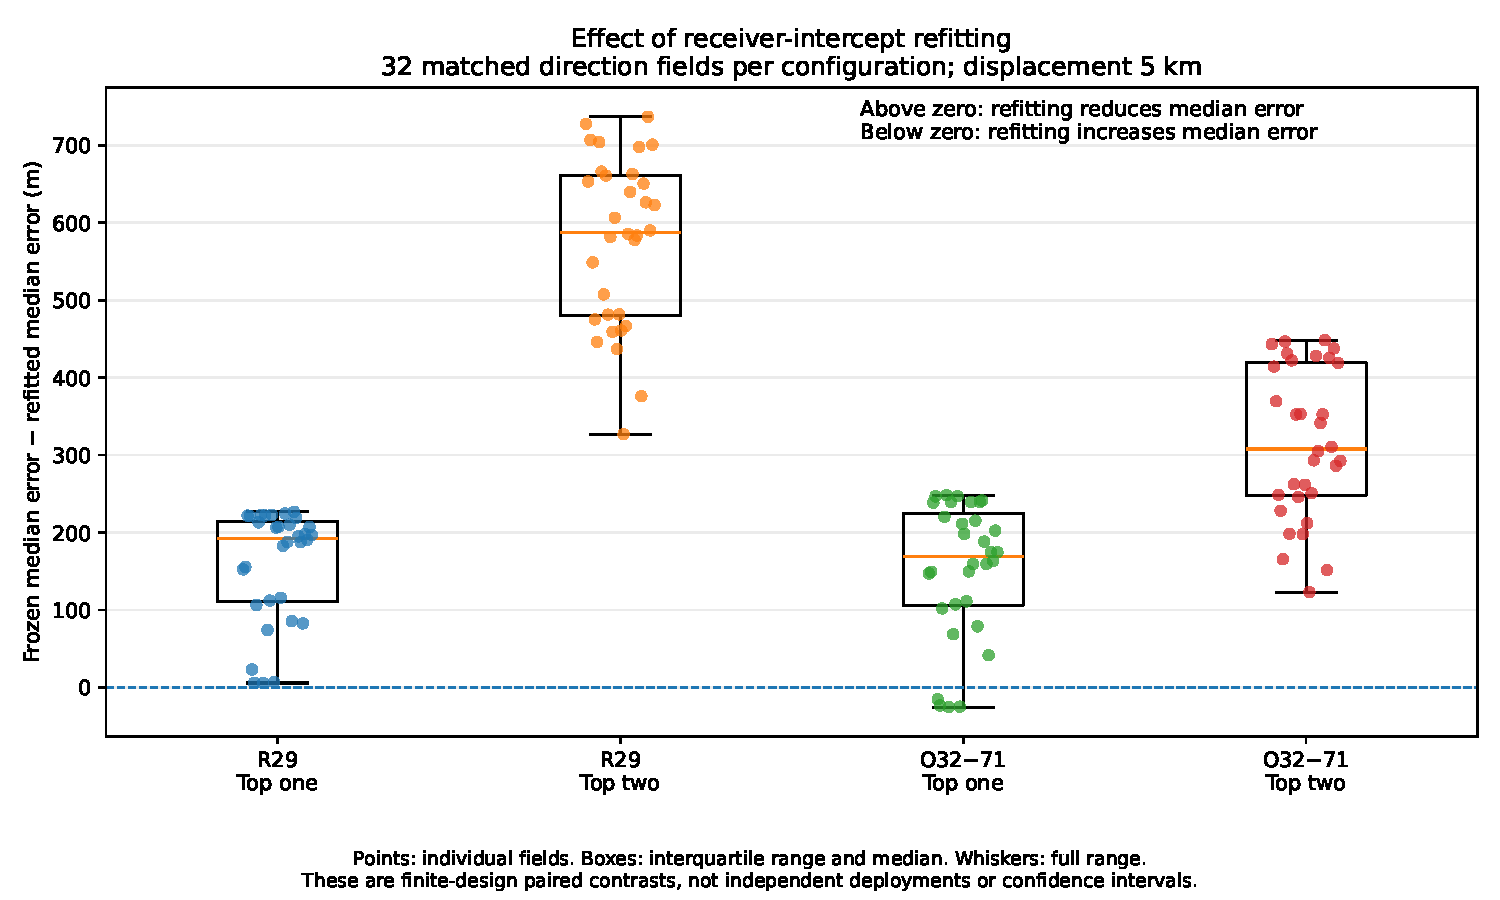
\includegraphics[width=0.95\textwidth]{figures/paired_calibration_32_fields.pdf}
\caption{Complete 32-field paired extension. Points and full ranges retain all four adverse O32$-$71 top-one cases. Boxes indicate medians and interquartile ranges, not confidence intervals.}\label{fig:s17paired}\end{figure}
\begin{figure}[htbp]\centering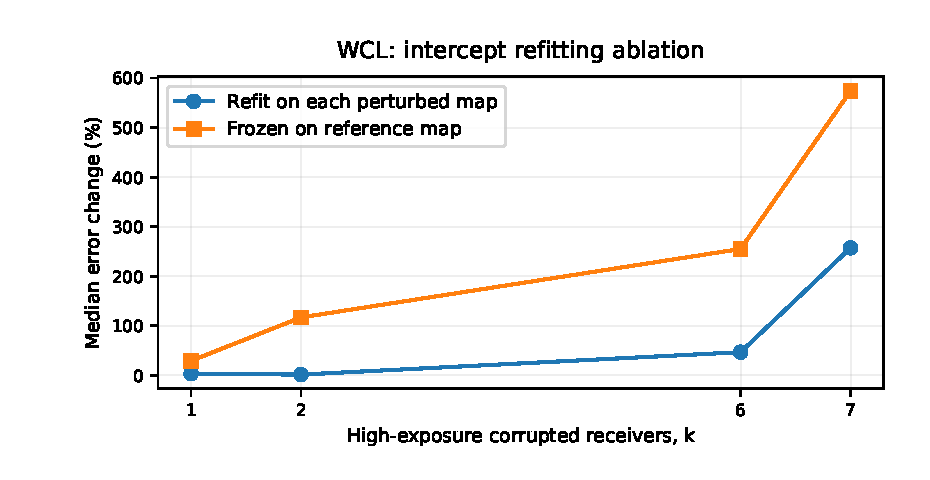
\includegraphics[width=0.8\textwidth]{figures/Fig4_A0_Refit_Ablation.pdf}
\caption{Historical two-field calibration ablation from S5. It is preserved as a separate record and is not the 32-field summary.}\label{fig:s17historical}\end{figure}

\clearpage
\section*{S18. Pooled Percentile Profile}
The original figure below accompanies the unchanged S8.2 quantile table. It was relocated from the main article to reduce competition with the principal contribution. Its numerical content and interpretation are unchanged: pooled marginal quantiles do not identify harmed-message subgroups, and 9992 denotes repeated evaluations of 2498 messages, not independent observations.
\begin{figure}[htbp]\centering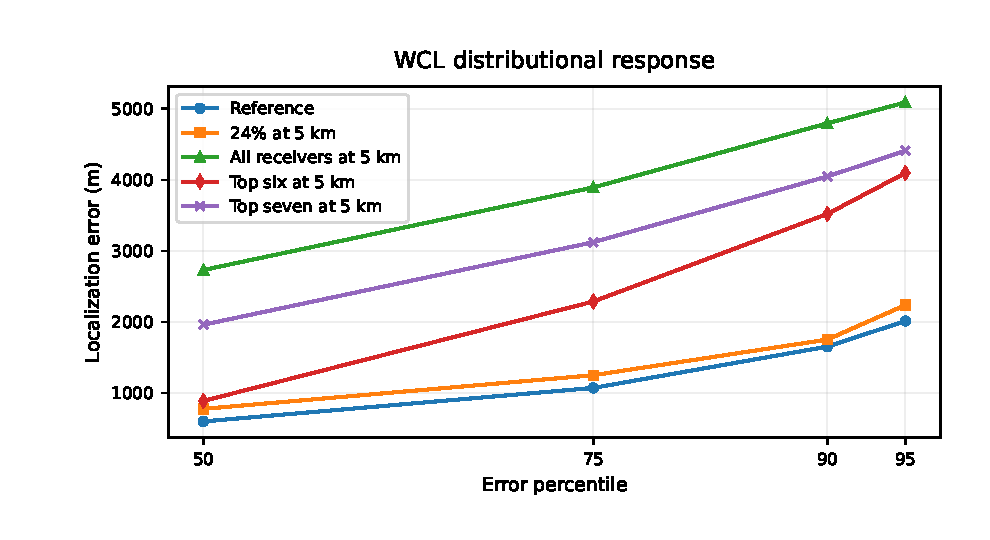
\includegraphics[width=0.85\textwidth]{figures/Fig7_Reliability_Profile.pdf}
\caption{Pooled WCL quantile profile. Top-six to top-seven increments are 1073~m at P50, 528~m at P90 and 312~m at P95. No individual-message or subgroup claim follows from these marginal summaries.}\label{fig:s18tails}\end{figure}

\end{document}
